% !TeX document-id = {54177b55-cdde-488b-90fe-107922d59049}
\documentclass[12pt]{article}

\usepackage{a4} 
\usepackage{amsmath}
\usepackage{amssymb}
\usepackage[]{xcolor}
\usepackage{graphicx}
\usepackage[colorlinks,urlcolor=blue,linkcolor=blue,citecolor=hotpink]{hyperref}
\usepackage{booktabs}
\usepackage{rotating}
\usepackage{caption}
\usepackage[british]{babel}
\usepackage[linesnumbered, ruled]{algorithm2e}
\usepackage{epstopdf}
\usepackage{mathtools} % for :=
\usepackage{subfig}
\usepackage[most, minted]{tcolorbox}
\usepackage{mdwlist}
\usepackage{multirow}
\tcbuselibrary{listings}

\newtcblisting{myminted}{%
	listing engine=minted,
	minted language=python,
	listing only,
	breakable,
	enhanced,
	minted options = {
		linenos, 
		breaklines=true, 
		breakanywhere, 
		fontsize=\footnotesize, 
		numbersep=2mm,
		tabsize=2
	},
	overlay={%
		\begin{tcbclipinterior}
			\fill[gray!25] (frame.south west) rectangle ([xshift=4mm]frame.north west);
		\end{tcbclipinterior}
	}   
}
\BeforeBeginEnvironment{minted}{\begin{tcolorbox}[breakable, enhanced]}%
	\AfterEndEnvironment{minted}{\end{tcolorbox}}%


\graphicspath{{images/}}

\title{Estimating the makespan of a stochastic schedule} % Think of a better title...
\author{Thomas McSweeney%
	\thanks{%
		School of Mathematics,
		University of Manchester,
		Manchester, M13 9PL, England
		(\texttt{thomas.mcsweeney@postgrad.manchester.ac.uk}).
	}
}
\date{\today}

%%%%%%%%%%%%%%%%%%%%%%%%%%%%%%%%%
\def\R{\mathbb{R}}
\def\C{\mathbb{C}}
\def\P{\mathbb{P}}
\def\E{\mathbb{E}}
\def\nbyn{n \times n}
\def\mbyn{m \times n}
\def\l{\lambda}
\def\norm#1{\|#1\|}      
\def\normi#1{\|#1\|_1}
\def\normo#1{\|#1\|_{\infty}}
\def\Chat{\widehat{C}}
\def\e{eigenvalue}
\DeclareMathOperator*{\argmax}{arg\,max}
\DeclareMathOperator*{\argmin}{arg\,min}
\def\diff{\mathop{}\!\mathrm{d}}

% \DeclareMathOperator{\diag}{diag}   % Requires amsmath.
\def\diag{\mathop{\mathrm{diag}}}     % If not using amsmath.
\def\trace{\mathop{\mathrm{trace}}}   % If not using amsmath.

\def\At{\widetilde{A}}
\def\normt#1{\|#1\|_2}

% Set up lemma environment and its numbering.
\newtheorem{lemma}{Lemma}[section]

\def\proof{{\bf Proof}. \ignorespaces}
\def\qedsymbol{\vbox{\hrule\hbox{%
			\vrule height1.3ex\hskip0.8ex\vrule}\hrule}}
\def\endproof{\qquad\qedsymbol\medskip\par}

\newtheorem{theorem}{Theorem}
\newtheorem{prop}[theorem]{Proposition}

\allowdisplaybreaks[1]

%%%%%%%%%%%%%%%%%%%%%%%%%%%%%%%%%%%%%%%%%%%%%%%%%%%%%%%%%%%%%%%%%%%%%%%%%%%%
% For fine-tuning spacing in \sqrt etc=.  From \cite[p.~155]{knut99}.
% In math mode, @ will act as a macro that adds 1 unit of space.
% By comparison, \, skips 3mu.

\mathcode`@="8000 % Make @ behave as per catcode 13 (active).  TeXbook p. 155.
{\catcode`\@=\active\gdef@{\mkern1mu}}
%%%%%%%%%%%%%%%%%%%%%%%%%%%%%%%%%%%%%%%%%%%%%%%%

%%%%%%%%%%%%%%%%%%%%%%%%%%%%%%%%%%%%%%%%%%%%%%%%%%%%%%%%%%%%%%%%%%%%%%%%%%%%
\newcounter{mylineno}
\makeatletter
\let\oldtabcr\@tabcr
\def\nonumberbreak{\oldtabcr\hspace{3.5pt}}
\def\mynewline{\refstepcounter{mylineno}%
	\llap{\footnotesize\arabic{mylineno}\hspace{5pt}}%
}
\def\lineref#1{\footnotesize\ref{#1}}
% Next macro adapted from latex.ltx
\gdef\@tabcr{\@stopline \@ifstar{\penalty%
		\@M \@xtabcr}\@xtabcr\mynewline}
\def\myvspace#1{\oldtabcr[#1]\mynewline}
\newenvironment{code}{%
	% Swap `:' and `colon'...
	\mathcode`\:="603A  % TeXbook pp 134, 154, 359 (top)
	% For original colon     \mathcode`\:="303A  % TeXbook p 344
	\def\colon{\mathchar"303A}
	\setcounter{mylineno}{0}
	\par
	\upshape
	\begin{list} % To give indentation
		{} {\leftmargin = 1cm}
		\item[]
		\begin{tabbing}
			
			% Default tab stops
			\hspace*{.3in} \= \hspace*{.3in} \=
			\hspace*{.3in} \= \hspace*{.3in} \= \kill
			\mynewline
		}{\end{tabbing}\end{list}}
\makeatother


\addto\captionsbritish{	\renewcommand{\bibname}%
	{References}%TODO: make sure reference style is consistent.
}

\definecolor{hotpink}{rgb}{0.9,0,0.5}

\begin{document}
	\maketitle 	


\section{Introduction}
\label{sect.intro}

% Questions for Neil: longest path or makespan throughout?

For any optimization problem, we obviously need to be able to evaluate how good any given solution is with regards to the optimization criteria in order to find an optimal, or otherwise acceptable, solution. The scheduling problems we consider here are clearly no exception: we want to know how good a computed schedule is, whether there are other schedules which are better, and so on. Evaluating the makespan of a given schedule would appear to be a straightforward problem---and so it is, when the computation and communication costs are static. But if costs are {\em stochastic} then this may no longer be the case.

Now, as long as it specifies the execution order of tasks on processors, any schedule $\pi$ for an application with task DAG $G$ can be represented by a {\em schedule graph} $G_{\pi}$ such that the longest path of $G_{\pi}$ is equal to the makespan of $\pi$: $G_\pi$ contains all the same vertices and edges as $G$, plus additional zero-weight {\em disjunctive} edges that indicate the execution order of the tasks on their chosen processors; the other weights of $G_\pi$ are induced by the processor selections of $\pi$. There's some flexibility in how we add the disjunctive edges; the most straightforward way to do it is to simply add an edge between a task $t_i$ and the task $t_h$ which is executed immediately before $t_i$ on its chosen processor if an edge does not already exist between the two.  
% We can interpret the entire scheduling problem as a question of how to add disjunctive edges such that the longest path is minimized...

For example, consider the schedule $\pi$ from Figure X and the graph $G$ in Figure Y. We can construct the associated graph $G_\pi$ as shown in Figure Z. From now, we use the notations $\pi_i$ and $\pi_{ik}$ to represent the computation cost of task $t_i$ and the communication cost between tasks $t_i$ and $t_k$ under the schedule $\pi$, respectively. Assuming, without loss of generality, that there is only one entry task $t_1$ and one exit task $t_n$, to compute the longest path through $G_\pi$---and therefore the makespan of $\pi$---we compute a sequence of numbers $L_i$ defined by $L_1 = \pi_1$ and
\begin{align}
  \label{eq.Li}
  L_i = \pi_i + \max_{h \in P_i}\{ \pi_{hi} + L_h\}
\end{align}
for all other $i = 2, \dots, n$. The longest path of $G_\pi$ is then given by $L_n$. In the example above, we have... so we see that $L_n$ is indeed equal to the schedule makespan. Computing the longest path using \eqref{eq.Li} is an $O(n + e) \approx O(n^2)$ operation, which depending on the size of the DAG may be expensive but is at least polynomial. (Of course, we could work backward through the DAG by setting $L_n = \pi_n$ and doing the maximization over the set of task children in \eqref{eq.Li} instead; the makespan would then be given by $L_1$ but the procedure is otherwise equivalent.)

Unfortunately, in practice, schedule costs are almost never known precisely before runtime. Typically, the best we can do is estimate the probability distribution that we believe they follow---i.e., we model the costs as random variables (RVs)---based either on theoretical results or a relevant body of data. But if costs are RVs rather than fixed scalars, it is obviously impossible to specify the precise time at which each task should begin execution so at this point we need to redefine what we mean by a schedule: here, we assume that a schedule $\pi$ is a mapping from tasks to processors that specifies only which tasks each processor should execute and in what order; the processor then executes the next scheduled task as soon as it is able. Conceptually, we can view this as a processor being assigned an ordered queue of tasks before runtime and only being allowed to pop the task currently at the head of the queue. 

This definition means that even though costs are stochastic, the disjunctive graph $G_\pi$ has the same topology as it would in the static case. However, since all costs are RVs, the longest path is also now an RV. Unfortunately, it is unclear how we should go about computing its distribution. Fundamentally, the problem is that even if all of the graph weights are independent of one another, path lengths typically aren't because of common nodes and edges. So if we attempt to apply \eqref{eq.Li} we soon run into difficulty because computing the maximum of a set of dependent RVs is intractable, with very rare exceptions. Furthermore, this presupposes that all individual cost distributions (and summations thereof) are fully known, which is rarely true in practice. Formalizing this intuitive difficulty, Hagstrom proved that computing the longest path distribution of a stochastic graph, or even just its expected value, is a $\#P$-complete problem when all weights are discrete RVs \cite{hag88}, and there is little reason to assume it is any easier in the continuous case.      

Given the difficulty of the problem, bounds or heuristic approximations for the longest path distribution---and therefore the schedule makespan distribution---are typically needed instead. In this chapter, we give a brief overview of various methods that have been employed for this purpose, with a particular focus on a family of efficient heuristics which are likely the most practical approach in the context of stochastic scheduling. Although useful on its own merits, in the context of this research this chapter functions as a bridge between earlier chapters which focus on computing schedules when costs are assumed to be known exactly and the later chapters in which the aim is to compute a schedule that is robust to the effects of uncertain cost estimates. We will see that many of the techniques discussed here underlie both existing stochastic scheduling heuristics and the new heuristic that we propose in the next chapter. This chapter is intended primarily as an literature review so there is relatively little new research, although we do take an extended look at a problem that has rarely been addressed before: how do we quickly update a longest path estimate---i.e., an estimated schedule makespan---as realizations become apparent at runtime? 

The problem of computing the distribution of the longest path through a DAG with stochastic weights was first studied in the context of {\em program evaluation review technique} (PERT) network analysis \cite{mal59}. Since a PERT network is essentially just what we have referred to here as a schedule graph, the longest path also typically represents an overall finish time---i.e., the makespan---and nodes tasks that must be completed. However, the stochastic longest path problem has also been studied in more dissimilar research areas such as digital circuit design \cite{bla08}, so in this chapter we typically use the more general {\em longest path} rather than {\em makespan}.  
% better reference for digital circuit design? 

\section{Bounds}
\label{sect.bounds}

Although computing the longest path distribution exactly is usually impossible, bounds on various quantities of interest may be computed much more cheaply. Depending of course on the context, these may be tight enough to be useful.

Some of the oldest results are concerned with the expected value. In particular, as we have already seen in previous chapters, a lower bound which dates back to the earliest days of PERT analysis can be computed in $O(n^2)$ operations by replacing all weight RVs with their expected value and proceeding as in \eqref{eq.Li}---i.e., define $u_1 = \E[\pi_1]$ and
\begin{align}
  \label{eq.ui}
  u_i = \E[\pi_i] + \max_{h \in P_i}\{ \E[\pi_{hi}] + u_h\}
\end{align}
for all other $i = 2, \dots, n$, then we have $u_i \leq \E[L_i]$ and in particular $u_n \leq \E[L_n]$. We will refer to this as the {\em critical path method} (CPM) bound. Furthermore, we also saw in the previous chapter that a tighter bound can be found through Fulkerson's \cite{ful62} alternative method, which was extended to continuous weights by Clingen \cite{cli64} and later improved by Elmaghraby \cite{elm67}. Although this approach as generalized by Robillard and Trahan \cite{rob76} can tighten the lower bound almost arbitrarily, the computational cost of even Fulkerson's bound can be prohibitive in some cases, as suggested by our experience in the previous chapter.    
% cpm bound since that was the context in which...

All of those methods provide only lower bounds for the expected value. However, Dodin's lower bound on the distribution function also induces an upper bound on the expected value \cite{dod85} (see below).  Furthermore, if all graphs weights follow {\em New Better Than Used in Expectation} (NBUE)\footnote{A concept from reliability theory, referring to distributions representing object lifetimes such that, at any given time, the expected value of the remaining lifetime is smaller than the expected value of the entire lifetime. Certain common distributions such as Erlang and uniform are NBUE, as are many others such as Gamma under restricted parameter regimes.} distributions, then an upper bound can be computed by replacing all weights by exponentially distributed RVs with the same means and then performing a series-parallel reduction \cite{kam85a, yaz91}. This approach has the advantage that only the expected values of all graph weights are necessary. 

Alternatively, if all node and edge weights are normally distributed, then Kamburowski \cite{kam85} was able to prove both lower and upper bounds on the expected value. However, his bounds---although exact when weights are normal---are conceptually very similar to a class of heuristics discussed in the following section, so will be described in more detail there. Kamburowski also proved a lower bound on the variance, as well as a conjectured upper bound, for the case of normally distributed weights. These are the only formal bounds on moments higher than the first that we are aware of, although the upper is unproven and the lower is very loose.

Rather than just the moments, we may be more interested in bounds on the cumulative distribution function (cdf) $F_{L_n}$ of the longest path, where the bounds indicate (first-order) {\em stochastically dominant} relationships between the underlying RVs. In particular, we say that $B$ stochastically dominates $L_n$ if $F_{L_n}(z) = \P[L_n \leq z] \leq \P[B \leq z] = F_B(z) \; \forall z$. For convenience, from now on we simply write $F_{L_n} \leq F_B$ to represent the previous expression, so that the aim here is to determine $F_b$ and $F_B$ such that $F_b \leq F_{L_n} \leq F_B$.

The first bounds on the distribution of the longest path were provided by Kleindorfer \cite{kle71}. Now, distribution functions for the sum and maximization of {\em independent} random variables are easily computed. In particular, suppose $X$ and $Y$ are independent and define $S = X + Y$ and $M = \max(X, Y)$. Then $F_S$ is computed through the convolution
\begin{align}
  \label{eq.cdf_convolution}
  F_S(z) = \int_{-\infty}^{\infty} F_Y(z - t) f_X(t) \; \diff t,
\end{align}
where $f_X$ is the probability density function of $X$, and $F_M$ via the product
\begin{align}
  \label{eq.cdf_product}
  F_M(z) = F_X(z) \times F_Y(z),
\end{align}
both of which can be readily approximated through standard numerical methods. Kleindorfer's upper bound is determined by working through the graph in the usual manner and assuming path independence---i.e., computing \eqref{eq.Li} using \eqref{eq.cdf_convolution} and \eqref{eq.cdf_product} for sums and maximizations, respectively. A corresponding lower bound is given by effectively disregarding all maximizations and simply using one of the operands.

Inspired by the observation that Kleindorfer's upper bound is exact when all path lengths are independent, Dodin \cite{dod85} combined the method with a sequence of series-parallel reductions such that the graph is transformed to a single edge whose associated distribution function bounds the longest path distribution from above. If the graph is already series-parallel then the bound is exact. Moreover, Dodin showed that the bound is tighter than Kleindorfer's, and, as noted above, that a corresponding lower bound on the expected value can be inferred.

Exhaustive empirical investigations by Ludwig, M{\"o}hring and Stork \cite{lud01} and Canon and Jeannot \cite{can16} suggest that the bounds of Kleindorfer and especially Dodin are usually tight, so they may be useful as approximations of the distribution function in addition to bounds. However, although both methods run in polynomial time, they tend to still be significantly more expensive than heuristics based on the Central Limit Theorem (see Section \ref{subsect.normality}), without pronounced improvements in accuracy, so are typically of less interest from a scheduling perspective and are not included in comparisons here. 

%Reference to Bein? Shogan?
%good reference for stochastic dominance.

\section{Heuristics}
\label{sect.heuristics}

Rather than a formal bound, in many cases it may be more useful to simply obtain a good estimate of the longest path distribution. To that end, many heuristic approaches have been proposed. In this section we discuss some of those which may be of particular interest.

\subsection{Monte Carlo}
\label{subsect.monte_carlo} 

% MC part is same as in previous chapter - where best to put it?

{\em Monte Carlo} (MC) methods have a long history in approximating the longest path distribution of PERT networks, dating back to at least the early 1960s \cite{van63}. The idea is to simulate the realization of all weight RVs and then evaluate the longest path of the resulting scalar graph. This is done repeatedly, giving a set of longest path instances whose empirical distribution function is guaranteed to converge to the true distribution by the Glivenko-Cantelli theorem\footnote{Despite this convergence in the limit, we refer to MC as a heuristic as any solutions obtained in practice will only ever be approximate.}. Furthermore, analytical results allow us to (at least roughly) quantify the approximation error for any given the number of realizations---and therefore the number of realizations needed to reach a given accuracy. On top of these theoretical assurances, the other big advantage of this approach is its simplicity: once the graph weights are realized, we only need to perform sums and maximizations of scalar values, rather than possibly dependent RVs.  
% Canon reference in support of the convergence claim? 

The major disadvantage of MC methods is the computational cost. Of course, modern architectures are well-suited to this approach because of their parallelism, but MC can still be impractical for large, dense graphs that require many realizations in order to obtain an accurate solution. For this reason, in our numerical experiments we typically only use MC to obtain a reference solution for the longest path distribution of a given schedule graph. 
% We call it a heuristic since the solutions are not exact by definition, although we do use them as a reference since they are guaranteed to converge...


\subsection{Applying the CLT}
\label{subsect.normality}

Fundamentally, the length of any given path through a schedule graph is just the sum of the weight RVs along it. By the Central Limit Theorem (CLT), sums of random variables are asymptotically normally distributed. So we can make a reasonable argument that the longest path distribution itself is likely to be at least approximately normal, $L_n \approx N(\mu_n, \sigma_n)$. Indeed, this has often been observed empirically, even when the graph weights follow distributions that are far from normal \cite{can10}. This argument forms the basis of a family of efficient heuristics for computing an approximation to the longest path distribution.

\subsubsection{Clark's equations and Sculli's method}
\label{subsubsect.clark_sculli}

Computing the longest path ultimately reduces to performing summations and maximizations of dependent random variables. If we assume that all weight RVs can be characterized by their mean and variance (i.e., effectively that they are also normal), then sums can be computed though the well-known rule for any two normal RVs $\epsilon \sim N(\mu_\epsilon, \sigma_\epsilon^2)$ and $\eta \sim N(\mu_\eta, \sigma_\eta^2)$,
\begin{align}
\label{eq.sum_moments}
\epsilon + \eta \sim N \big(\mu_\epsilon + \mu_\eta, \sigma_\epsilon^2 + \sigma_\eta^2 + 2 \rho_{\epsilon\eta}\sigma_\epsilon \sigma_\eta \big), 
\end{align}
where $\rho_{\epsilon\eta}$ is the linear correlation coefficient between the two distributions. Formulae for the first two moments of the maximization of two normal RVs---which is not itself normal---are less well-known but were first provided by Clark in the early 1960s \cite{cla61}. Let 
\begin{align*}
\phi(x) = \frac{1}{\sqrt{2\pi}} e^{-x^2/2} \quad \text{and} \quad \Phi(x) = \int_{-\infty}^{x} \phi(t) dt
\end{align*}
be the unit normal probability density function and cumulative probability function, respectively, and define 
\begin{align}
  \label{eq.alpha_beta}
\alpha = \sqrt{\sigma_\epsilon^2 + \sigma_\eta^2 - 2 \rho_{\epsilon\eta}\sigma_\epsilon \sigma_\eta} \quad \text{and} \quad \beta = \frac{\mu_\epsilon - \mu_\eta}{\alpha}. 
\end{align}
Then the first two moments $\mu_{\max}$ and $\sigma_{\max}$ of $\max(\epsilon, \eta)$ are given by
\begin{align}
\mu_{\max} &= \mu_\epsilon \Phi(\beta) + \mu_\eta \Phi(-\beta) + \alpha \phi(\beta), \label{eq.clark_max_mu}\\
\sigma_{\max}^2 &= (\mu_\epsilon^2 + \sigma_\epsilon^2) \Phi(\beta) + (\mu_\eta^2 + \sigma_\eta^2) \Phi(-\beta) \label{eq.clark_max_sigma}\\
&+ (\mu_\epsilon + \mu_\eta)\alpha\phi(\beta) -\mu_{\max}^2 \nonumber.
\end{align}
Although these formulae are exact, they are only valid for a single pair of normal RVs. As already noted, the maximization of two normal RVs is not normal, so we cannot obtain the exact moments for a set of arbitrarily many RVs by applying them in a pairwise manner. However, we can at least get an approximation. Sinha, Zhou and Shenoy \cite{sin07} empirically investigated the accuracy of this approximation for sets of up to 100 normal RVs, concluding that it is usually fairly good. Furthermore, they considered several possible orderings for the operands of the maximization (randomly, by mean value, and so on), a topic that was also briefly discussed by Ross \cite{ross03}.        

Bringing this all together, by using \eqref{eq.sum_moments} for summations, and \eqref{eq.clark_max_mu} and \eqref{eq.clark_max_sigma} pairwise for maximizations, we can now move through the graph in a manner similar to \eqref{eq.Li} and compute approximations $\mu_n$ and $\sigma_n^2$ to the first two moments of the longest path which, since it is assumed to be roughly normal, suffices to describe the entire distribution. This method appears to have first been proposed for estimating the completion time of PERT networks by Sculli \cite{scu83}, although to simplify the problem he assumed that all of the correlation coefficients $\rho_{\epsilon \eta}$ in \eqref{eq.alpha_beta} were zero (see next section).

In practice, the moment estimates obtained using Sculli's method tend to be quite accurate, with performance improving as the weight distributions move closer to normality and the number of nodes in the graph increases (as we might intuitively expect). More importantly, Sculli's method is typically much faster than the alternatives \cite{can16}. 

\subsubsection{Including correlations}
\label{subsubsect.correlation_aware}

Sculli assumed that all correlations were zero, which is rarely the case in practice since common ancestors make the longest path at two nodes dependent, even if all weights themselves are independent. Computing the correlation coefficients efficiently is tricky. However, Canon and Jeannot \cite{can16} proposed two different heuristics which alternatively prioritize precision and speed. The first is a dynamic programming algorithm called Cordyn which recursively computes the correlations using formulae derived in Clark's original paper for the correlation coefficients between any normal RV $\tau$ and a summation or maximization of normal RVs $\epsilon$ and $\eta$, 
\begin{align}
  \label{eq.clark_corrs}
  \rho_{\tau, \, \text{sum}(\epsilon, \eta)} &= \frac{\sigma_\epsilon \rho_{\tau \epsilon} + \sigma_\eta \rho_{\tau \eta} }{\sigma_{\text{sum}}} \quad \text{and} \quad
\rho_{\tau, \max(\epsilon, \eta)} = \frac{\sigma_\epsilon \rho_{\tau \epsilon} \Phi(\beta) + \sigma_\eta \rho_{\tau \eta} \Phi(-\beta)}{\sigma_{\max}}.
\end{align} 
Cordyn has time complexity $O(ne) \approx O(n^3)$, so is more expensive than Sculli's method, which is quadratic in $n$, but numerical experiments performed by Canon and Jeannot suggest that it is almost always more accurate. 
% something about being competitive with reduction based methods?

In an effort to marry the speed of Sculli's method and the accuracy of Cordyn, Canon and Jeannot also proposed an alternative heuristic called CorLCA. The main idea is to construct a simplified version of the DAG called a {\em correlation tree} that has all the same nodes as the original but only retains a subset of the edges. In particular, where multiple edges are incident to a node---i.e., a maximization must be performed---only the edge which contributes most to the maximization is retained in the correlation tree. The motivation here is that the correlation coefficient between any two longest path estimates $L_i$ and $L_k$ can be efficiently approximated by finding the {\em lowest common ancestor} (LCA) $t_{a}$ of the corresponding nodes $t_i$ and $t_k$ in the correlation tree: since $L_i \approx L_a + \eta$ and $L_k \approx L_a + \epsilon$ where $\eta$ and $\epsilon$ are independent RVs representing the sums of the costs along the paths between $t_a$ and $t_i$ (resp. $t_a$ and $t_k$) in the correlation tree, we have
\begin{align*}
  \rho_{L_i, L_k} \approx \frac{\sigma_{L_a}^2}{\sigma_{L_i}\sigma_{L_k}}. % Not technically correct---introduce C?
  \end{align*}
  For every edge, we need to do a lowest common ancestor query, so the time complexity of CorLCA depends to a large extent on the cost of these. Although they do not present a method, based on similar results in the literature, Canon and Jeannot hypothesize this can be done in $O(1)$ operations, giving an overall time complexity $O(e) \approx O(n^2)$ for the entire algorithm. At any rate, an extensive numerical comparison of several heuristic methods for approximating the longest path distribution by the original authors suggested that CorLCA is more efficient than Cordyn with only a relatively small reduction in accuracy \cite{can16}. It should however also be noted that it can do badly when longest path length estimates at two or more nodes with a common child are similar since only one of the respective edges to the child will be retained in the correlation tree.

  \subsubsection{The canonical method}
\label{subsubsect.canonical}


Another method for estimating the longest path distribution that approximates correlations in a similar manner comes from the field of digital circuit design. In the so-called {\em canonical model} \cite{vis06,zha06}, all RVs are expressed as the sum of their expected value and a weighted sum of standard normal distributions that characterize the variance, 
\begin{align*}
\eta = \mu + \sum_i v_i \delta_i,
\end{align*}  
where all $\delta_i \sim N(0, 1)$ and are independent of one another. The advantage of this is that evaluating summations and maximizations becomes much more straightforward. Let $\eta = \mu_\eta + \sum_i v_{\eta, i} \delta_i$ and $\epsilon = \mu_\epsilon + \sum_i v_{\epsilon, i} \delta_i$. Then 
\begin{align*}
\omega = \eta + \epsilon = (\mu_\eta + \mu_\epsilon) + \sum_i (v_{\eta, i} + v_{\epsilon, i}) \delta_i.
\end{align*}
Suppose now that $\omega = \max(\eta, \epsilon)$. Let $\alpha$ and $\beta$ be defined as in \eqref{eq.alpha_beta}, and $\Phi(x) = \int_{-\infty}^{x} \phi(t) dt$ be the standard normal cdf. Note that computing $\beta$ requires the linear correlation coefficient $\rho_{\eta\epsilon}$ which can be efficiently calculated as:
\begin{align*}
\rho_{\eta\epsilon} = \frac{\sum_i v_{\eta, i} v_{\epsilon, i}}{\sqrt{\sum_i v_{\eta, i}^2} \cdot \sqrt{\sum_i v_{\epsilon, i}^2} }.
\end{align*}
By definition, $\P[\eta > \epsilon] = \Phi(\beta)$ and we can therefore approximate $\omega$ by 
\begin{align*}
\hat{\omega} &= \Phi(\beta)\eta + \Phi(-\beta) \\
&= \Phi(\beta) \mu_\epsilon + \Phi(-\beta) \mu_\epsilon + \sum_i \big( \Phi(\beta) v_{\eta, i} + \Phi(-\beta) v_{\epsilon, i} \big) \delta_i.
\end{align*}
This is both similar and in some sense contrary to the Clark equation approach, in that the latter precisely computes the first two moments of the maximization of two normal RVs, whereas the canonical method approximates the distribution of the maximization of any two RVs using linear combinations of normal RVs. In their empirical comparison, Canon and Jeannot found that the canonical method tended to fall between Sculli's heuristic and CorLCA in terms of both speed and approximation quality \cite{can16}, so we decided not to include it in comparisons here. 


\subsubsection{Kamburowski's bounds}
\label{subsubsect.kamburowski}

As stated in Section \ref{sect.bounds}, when all costs are independent Gaussian RVs, Kamburowski was able to prove both upper and lower bounds on the first two moments\footnote{As noted previously, the upper bound on the variance technically remains a conjecture.} of the longest path distribution. Since the bounds are somewhat similar to the methods discussed elsewhere in this section, we describe them here.

The basic idea is to recursively compute four number sequences $\underline{m_i}$, $\overline{m_i}$, $\underline{s_i}$ and  $\overline{s_i}$ such that $\underline{m_i} \leq \mu_{L_i} \leq \overline{m_i}$ and $ \underline{s_i} \leq \sigma_{L_i} \leq \overline{s_i}$ for all $i = 1, \dots, n$. Clearly, by taking $\underline{m_1} = \overline{m_1} = \E[\pi_1]$ and $\underline{s_1}^2 = \overline{s_1}^2 = Var[\pi_1]$ we can achieve the desired bounds for $L_1$. (As ever, we could work backward instead, in which case the analogous results hold for the index $n$.) Now we suppose that all of the upper and lower bounds have been computed for all of the parents of a given node $t_i$ and consider how we can construct  $\underline{m_i}$, $\overline{m_i}$, $\underline{s_i}$ and  $\overline{s_i}$. The variance bounds are relatively straightforward, albeit loose. The lower bound is given by
\begin{equation}
\underline{s_i^2} =\left\{
\begin{array}{@{}ll@{}}
\underline{s_h^2} + Var[\pi_{hi}] + Var[\pi_{i}], \quad  \text{if $P_i = \{s_h\}$,} \\
0,  \quad \text{ otherwise},
\end{array}\right.
\label{eq.si_under}
\end{equation}
reflecting the intuition that the variance can be reduced almost arbitrarily by a maximization (which needs to be performed for the case of multiple parents). The upper bound is similarly intuitive since it is effectively equivalent to saying that the variance of the maximum of a set of normal RVs is bounded above by the maximum variance of the RVs, although this has never been proven (see Section \ref{subsect.discussion}). More precisely, define 
\begin{align}
  \label{eq.si_over}
  \overline{s_i^2} = \max_{h \in P_i}\{ \overline{s_h^2} + Var[\pi_{hi}] + Var[\pi_{i}]\}.
\end{align}
The bounds on the expected value are somewhat more complex. First, define a function $h$ by
\begin{align*}
  h(\mu_i, \sigma_i, \mu_k, \sigma_k) = \mu_i \Phi(\overline{\beta}) + \mu_k \Phi(-\overline{\beta}) + \overline{\alpha} \phi(\overline{\beta}),
\end{align*}
where $\overline{\alpha} = \sqrt{\sigma_i^2 + \sigma_k^2}$ and $\beta = (\mu_i - \mu_k)/ \overline{\alpha}$. Per equation \eqref{eq.clark_max_mu}, $h$ is the expected value of the maximization of two {\em independent} normally distributed RVs $X_i \sim N(\mu_i, \sigma_i^2)$ and $X_k \sim N(\mu_k, \sigma_k^2)$. Now, suppose that we have a set of (not necessarily independent) normally distributed RVs $X_1, X_2, \dots, X_r$, where each $X_i \sim N(\mu_i, \sigma_i^2)$ and $\sigma_1 \leq \sigma_2 \leq \dots \leq \sigma_r$. Define two functions $\underline{f}$ and $\overline{f}$ by the recursions,
\begin{align*}
  &\underline{f}(X_1) = \overline{f}(X_1) = \mu_1, \\
  &\underline{f}(X_1, X_2) = \overline{f}(X_1, X_2) = h(\mu_1, \sigma_1, \mu_2, \sigma_2), \\
  &\underline{f}(X_1, \dots, X_r) = h(\underline{f}(X_1, \dots, X_{r - 1}), 0, \mu_r, \sigma_r), \\
  &\overline{f}(X_1, \dots, X_r) = h(\overline{f}(X_1, \dots, X_{r - 1}), \sigma_{r - 1}, \mu_r, \sigma_r).
\end{align*}
Then, for all $i = 2, \dots, n$, if we define
\begin{align*}
  \underline{m_i} &= \underline{f}(\{ \underline{X_h} \}_{h \in S_i}),
\end{align*}
where
\begin{align*}
  \underline{X_h} &\sim N(\underline{m_h} + \E[\pi_{hi}] + \E[\pi_{i}], \; \underline{s_h^2} + Var[\pi_{hi}] + Var[\pi_{i}]),
\end{align*}
and
\begin{align*}
  \overline{m_i} &= \overline{f}(\{\overline{X_h}\}_{h \in S_i}),
\end{align*}
where
\begin{align*}
  \overline{X_h} \sim N(\overline{m_h} + \E[\pi_{hi}] + \E[\pi_{i}], \; \overline{s_h^2} + Var[\pi_{hi}] + Var[\pi_{i}]),
  \end{align*}
we have 
\begin{align*}
  \underline{m_i} \leq \mu_{L_i} \leq \overline{m_i}.
\end{align*}
(Here we are assuming that the sets $\{\underline{X_h}\}_{h \in S_i}$ and $\{\overline{X_h}\}_{h \in S_i}$ are ordered in such a way that the inequality constraints on the variances is satisfied.)

\section{A path-based heuristic}
\label{sect.path_heuristic}

By definition, the longest path through a graph is exactly that: the longest of all possible paths. Let $q$ denote the number of paths and $P_a$ be any path. Then we have
\begin{align}
  \label{eq.lp_definition}
  L_n = \max_{a = 1, \dots, q} P_a.
\end{align}
Since all path lengths are approximately normal by the CLT---or exactly normal if all weight distributions are as well---this reduces to the problem of finding the maximum of a set of dependent, differently distributed (DDD) normal RVs. Of course, the problem with this approach is that $q$ is usually impractically large; it is rare that we can even efficiently generate all of the possible paths, let alone evaluate their maximum. The dynamic programming approach defined by \eqref{eq.Li} is therefore (usually) the only possible option. In that case we also have to deal with finding the maximum of sets of normal path length RVs, but they are much smaller so we can apply Clark's equations in any of the flavors---Sculli's method, CorLCA, Cordyn---described previously. However, one potential downside is that approximation errors can propagate through the DAG. An illustration of this principle is provided by the fact that the longest path distribution computed by the forward and backward variants of Sculli's method and CorLCA can be quite different (see Section X). But if we could somehow reduce the set of paths that need to be considered to a smaller, more manageable size we could apply Clark's equations directly to the path lengths and hopefully alleviate this effect. In other words: can we identify a subset of paths that are (in some reasonable sense) the most likely to be the longest?

This problem has been considered before. For example, Dodin \cite{dod84} presented a polynomial time algorithm for determining the $K$ {\em most critical} paths in a PERT network, where criticality is defined in terms of the probability that a path will be greater than all others. A modified version of Dodin's algorithm was used by Ludwig, M{\"o}hring and Stork \cite{lud01} in conjunction with the normality assumption as a heuristic bound on the distribution function: paths were generated according to the algorithm and their length distributions were then multiplied together to (heuristically) bound the longest path distribution. As noted in Section \ref{sect.bounds}, this heuristic performed well in comparison to other methods, even though multiplying the path length distributions treats them as though they were independent.

We propose a very similar heuristic here that we call {\em Reduce Paths to Maximize} (RPM) for ease of reference. At a high level, it has the following two step structure:
\begin{enumerate}
\item Identify a set of paths that are good candidates to be the longest.
  \item Approximate the distribution of their maximization.
  \end{enumerate}
We describe our approach for both of these steps in more detail in the following two sections.

\subsection{Identifying longest path candidates}
\label{subsect.identifying}

Given any two paths $P_a \sim N(\mu_a, \sigma_a^2)$ and $P_b \sim N(\mu_b, \sigma_b^2)$ whose lengths are assumed to be normally distributed by the CLT, the probability that $P_a$ is greater than $P_b$ is given by
\begin{align}
  \label{eq.path_comparison}
  \P(P_a > P_b) = \Phi \bigg( \frac{\mu_a - \mu_b}{\sqrt{\sigma_a^2 + \sigma_b^2 - \rho_{ab}\sigma_a \sigma_b}} \bigg),
\end{align}
where $\rho_{ab}$ is the linear correlation coefficient between $P_a$ and $P_b$. Note that $\rho_{ab}$ can be efficiently estimated by letting $C \sim N(\mu_C, \sigma_C^2)$ be the sum of the shared node and edge weights, so that $\rho_{ab} \approx \sigma_C^2 / \sigma_a \sigma_b$. 
One immediate observation from \eqref{eq.path_comparison} is that if $\mu_a > \mu_b$ then $\P(P_a > P_b) > 0.5$, so the path with the greatest mean value is likely longer than any other given path through the graph (although not necessarily {\em all} other paths, a distinction best elucidated by Soroush \cite{sor94}). We use this simple fact as the basis for a method of generating a set of paths that are intuitively likely to be the longest.

For a given $\epsilon < 1$, we say that $P_a$ {\em $\epsilon$-dominates} $P_b$ if $\P(P_a > P_b) > 1 - \epsilon$. For all $i = 1, \dots, n$, define $P_i^*$ to be the path from the source to $t_i$ with the greatest expected value. Let $X_i$ be the set of all paths to $t_i$ which are {\em not} $\epsilon$-dominated by $P_i^*$---i.e., $P \in X_i \iff \P(P_i^* > P) < 1- \epsilon$. Suppose $t_k$ is a child of $t_i$. If $t_i$ is the only parent of $t_k$, then we simply define
\begin{align*}
  X_k = \{P + \pi_{ik} \mid P \in X_i\}.
\end{align*}
Things are slightly more complicated if $t_k$ has multiple parents: we need to identify $P_k^* \coloneqq \max_{h \in P_i} \{ \E[P_h^*] + \E[\pi_{hk}] \}$, then check all paths in the set  
\begin{align*}
  \cup_{h \in P_i}\{P + \pi_{hk} \mid P \in X_h \}
\end{align*}
and add those which are not $\epsilon$-dominated by $P_k^*$ to $X_k$. Moving forward through the graph in this manner, $X_n$ gives us our set of path candidates. Bringing this all together, Algorithm X summarizes the full procedure.    
 
Of course, it is very easy to construct examples for which this heuristic does badly, such as when we have many paths of similar length. For the sake of efficiency, it is sensible to set an upper limit on the number of paths that are retained at each node, but in the worst case this method can still be expensive (although it has polynomial time complexity). However, the hope is that computing the candidate paths is not too tedious for an average graph. Similarly, there are absolutely no theoretical guarantees that the generated paths are a useful substitute for the full set of paths. However, we investigate both of these conjectures via numerical experimentation in Section \ref{sect.results}. 

\subsection{Approximating the maximum}
\label{subsect.approx_max}

Once the set of candidate paths $X_n$ has been computed, we can estimate the distribution of their maximum using the Clark equations pairwise. The question then is, how do we deal with the correlations? Now, as noted above, correlations between any two given paths can be computed efficiently, so we could take a similar approach to CorLCA and use only the single dominant path in the intermediate maximizations in order to estimate the correlations. Alternatively, we could use \eqref{eq.clark_corrs} to recursively compute all of the correlation coefficients required for the maximization over the entire set, in a manner similar to Cordyn. We consider the empirical performance relative to their computational cost for both of these alternatives in Section \ref{sect.results}.  

\subsection{Discussion}
\label{subsect.discussion}

Given that we are essentially replacing \eqref{eq.lp_definition} with a maximization over a much smaller set of DDD normal RVs, certain results from the literature may now be applicable. Although much less studied than the independent, identically distributed (IID) case, bounds on both the distribution and its moments have been established, but none of these are practical for the full set of paths. However, although they technically no longer hold, they may be useful heuristically when applied to the subset of longest path candidates $X_n$ as defined above.

Ross gives a general upper bound for the expected value of a set of (not necessarily normal) DDD RVs, which he later specializes for the normal case, as well as mathematical programs for computing tight upper and lower bounds when the RVs are normally distributed \cite{ross03}. Their practical limit is stated to probably be for sets comprising hundreds of RVs, which may be feasible depending on the size of $X_n$. On the other hand, while Galambos \cite{gal72} presents bounds on the distribution it isn't clear how they can be practically computed even for small sets.

As an aside, it is interesting to note that when all weights are normal---so all paths are exactly normal as well---there is at least one bound we can prove even for the full set of path lengths. Since the mean of a given path length is just the sum of the means of the weights along it, we can easily find $\max_a(\E[P_a])$ via dynamic programming. This is useful because by Jensen's inequality we have  
  $\E[\max_aP_a] \geq \max_a(\E[P_a])$---i.e., the classic CPM lower bound on the expected value of the longest path. (Of course, this can be proven via other methods to be true even when all weights are not normally distributed.) Similarly, $\max_a(Var[P_a])$ can be computed cheaply for normal weights, which is Kamburowski's conjectured upper bound on the variance of the longest path in that case. The bound therefore holds if and only if
  \begin{align*}
    Var[\max(X_1, \dots, X_N)] \leq \max(Var[X_1], \dots, Var[X_N]),
  \end{align*}
  for any set of DDD normal RVs $X_1, \dots, X_N$. While simple counterexamples to this conjecture can be found for RVs from {\em arbitrary} distributions, as far as we know it remains an open question for normal RVs. In fact, if we assume that the shape of the maximum is roughly normal, since the mean of the maximum is greater than the mean of any path, we could argue heuristically that the variance of the longest path is actually bounded in the normal case by $Var[P_M]$, where   
\begin{align*}
    M \coloneqq \argmax_a(\E[P_a] + Var[P_a]).
 \end{align*}
 We briefly consider if this possible bound holds via numerical experiments described in Section \ref{sect.results}.
  
% QUESTION FOR NEIL.
  %Perhaps the best approach is to give up on exact bounds and take a heuristic approach. In particular, the following concentration inequality may be useful for (roughly) bounding the distribution function of the longest path...
  %\begin{prop}
%	Let $g = (g_1, \dots, g_n)$ be a Gaussian random vector, whose coordinates are not necessarily independent. One can express $g$ as... Let $\sigma^2 = \max_iVar(g_i)$. Then for all $t > 0$,
%	\begin{align*}
%	\P\bigg[\max_i g_i - \E[\max_i g_i] \geq t \bigg] \leq e^{-t^2/2\sigma^2}
%	\end{align*}
     %   and
     %   \begin{align*}
%	\P\bigg[\max_i g_i - \E[\max_i g_i] \leq -t \bigg] \leq e^{-t^2/2\sigma^2}.
%	\end{align*}
    %  \end{prop}  

% One speculative approach that might be useful is to consider extreme value theory... The problem is that it isn't clear how to characterize the distribution. Paper by Berman (and other one) seems to suggest that max of dependent normals will also tend to Gumbel but don't know anything about the correlations...

\section{Updating makespan estimates}
\label{sect.updating}

% Makespan or longest path? Have used LP earlier but makespan more sensible here...

Estimating the length of a schedule with stochastic costs before its execution has been widely-studied, as the examples in previous sections illustrate. However a related problem has received less attention: how can schedule makespan estimates be quickly updated {\em during} execution? This would be particularly useful in situations such as when a large unexpected delay occurs. More precisely, the scenario we consider is as follows. Given a schedule $\pi$, we have a complete set of task finish times estimates $L_i \sim N(\mu_i, \sigma_i^2)$ for all $i = 1, \dots, n$ that were computed before runtime. At some point in time $T$ during the schedule execution we want to compute a new estimate of the makespan based on the data gathered thus far. How do we do this as quickly and accurately as possible?

Effectively, at time $T$ the schedule graph $G_s$ can be divided into two distinct subgraphs: one corresponding to those tasks that have been completed and the other to those that have not. Define $C_T$ to be the set of indices corresponding to tasks that have completed by time $T$ and $U_T$ to be the set of indices corresponding to tasks that are still not done. Furthermore, define $C_T^* \subseteq C_T$ to be the set of indices of tasks which have been completed but at least one of their parents has not---in some sense the boundary of the realized and unrealized sections of the graph.
% something about the first having multiple exit tasks and the second multiple entry tasks?

Since all cost RVs corresponding to tasks indexed by $C_T$---and the edges between them---have been realized, we can compute the realized finish times $\ell_i$ for the corresponding tasks in the usual manner for scalar costs. The question then remains of how we compute an updated set of makespan estimates $L_k'$ for all $k \in U_T$, including a new final makespan estimate $L_n'$. We outline different possible approaches to this problem in the following three sections.

\subsection{Create a new graph}
\label{subsect.remaining}

The most straightforward approach is to simply consider the unrealized part of the graph separately and compute the longest path through it, starting from any of the boundary tasks indexed by $C_T^*$, using any method. A new longest path estimate which passes through the given boundary task is then the sum of the realized longest path up to and including the task, plus the estimated longest path through the remaining unrealized subgraph. More efficiently, rather than initially computing values $L_i$ that represent longest path lengths from the source to a task (inclusive), we can compute a sequences of values $R_i$ that represent the longest paths from the tasks to the sink (exclusive)---i.e., estimates of the remaining time until the entire schedule has been completed. In particular, we set $R_n = 0$, then work backward and recursively compute  
\begin{align*}
  R_i = \max_{k \in S_i} \{ \pi_{ik} + \pi_k + R_k  \}
\end{align*}
for all other tasks, where the maximization is approximated using any of the methods that have been discussed (or otherwise). Note that since the $R_i$ do not include the cost of task $t_i$ the schedule makespan estimate is actually $R_1 + \pi_1$.

(Of course, minor changes need to be made to some heuristics in order to estimate the correlations when working backward through the DAG. For example, in CorLCA, rather than the lowest common ancestors of two tasks, we want the deepest common descendants. However these changes are typically straightforward. As an aside, though, fairly significant differences are sometimes apparent between makespan estimates computed forward and backward through the DAG; see Section \ref{subsect.results_heuristics}.) 

The advantage of this approach is that at time $T$ the estimated longest path which passes through task $t_i$, where $i \in C_T^*$, is simply given by $L_i' = \ell_i + R_i$ and, in particular, a new estimate of the makespan can be computed through
\begin{align*}
  L_n' = \max_{i \in C_T^*} \{ \ell_i + R_i  \}.
\end{align*}
Correlations for this maximization can be estimated in the same manner as was done for the calculation of the $R_i$, ideally using the same set of correlation coefficients (or not, if using Sculli's method).

\subsection{Update the makespan directly}
\label{subsect.corr_update}

Another possible method for updating the final makespan estimate makes use of the following result.
\begin{prop}
	Let $u$ be a normally distributed vector with mean $\bar{\mu}$ and covariance $\Sigma_u$, $u \sim N(\bar{\mu}, \Sigma_u)$, and suppose that $u = (v, w)$. Then 
	\begin{align*}
	(w \mid v) \sim N \big( \bar{w} + \Sigma_{wv}\Sigma_{vv}^{-1} (v - \bar{v}), \enspace  \Sigma_{ww} - \Sigma_{wv} \Sigma_{vv}^{-1} \Sigma_{vw} \big).
	\end{align*}
\end{prop}
Note that if all of the linear correlation coefficients $\rho_{uv}$ are known, we can use the definition $\rho_{uv} = \Sigma_{uv} / \sigma_u \sigma_v$ to find $\Sigma_{uv}$.

This proposition is useful because we are assuming that there is a joint normal distribution across the entire set of finish times $L_i$. Furthermore, we can estimate the correlation coefficient between finish times at any two tasks using, for example, the correlation tree approach of CorLCA. This means that we can update the final makespan estimate using only the observed finish times of the tasks indexed by $C_T^*$. For compactness of notation let $\rho_{in} = \rho_{ni}$ be the linear correlation coefficient between $L_i$ and $L_n$. Suppose that task $t_i$ has finished at time $\ell_i$. Then we can compute a new estimate $L_n^i$ of the final makespan by applying the above result as follows,
\begin{align*}
L_n^i &\sim N \bigg( \mu_{n} + \frac{\rho_{ni} \sigma_{n} \sigma_{i}}{\sigma_{i}^2} (\ell_i - \mu_{i}), \enspace \sigma_{n}^2 - \frac{\rho_{ni} \sigma_{n} \sigma_{i} \cdot \rho_{in} \sigma_{i} \sigma_{n}}{\sigma_{i}^2} \bigg) \nonumber\\
&\sim N \bigg(\mu_{n} + \frac{\rho_{ni} \sigma_{n}}{\sigma_{i}} (\ell_i - \mu_{i}), \enspace (1 - \rho_{ni}^2) \sigma_{n}^2 \bigg).
\end{align*}
We do this for all $i \in C_T^*$ and then compute their maximum (using the same method as before to estimate the correlation coefficients, if they are not already known) in order to obtain a new estimated final makespan $L_n'$, 
\begin{align*}
  L_n' = \max_{i \in C_T^*} \{ L_n^i  \}.
  \end{align*}

\subsection{Do the computation again}
\label{subsect.propagating}

Rather than updating the finish time of the exit task---and therefore the makespan---directly, we can instead move forward through the DAG and update the finish time estimates for all unrealized tasks. This is more expensive of course but potentially more accurate. Now, in principle the updated finish times can be computed for each task $t_i$, where $i \in U_T$, using equation \eqref{eq.Li} in the usual manner. However, there are essentially three different cases that we need to consider, depending on the status of the terms in the maximization.
\begin{enumerate}
\item Both $\pi_{hi}$ and $L_h$ have been realized for all $h \in P_i$.
\item Both $\pi_{hi}$ and $L_h$ have been realized for some $h \in P_i$ but not others. 
  \item Both $\pi_{hi}$ and $L_h$ have been realized for none of the parents.
  \end{enumerate}
  In the first instance, the sums of $\pi_{hi}$ and $L_h$ are now deterministic so the maximization is just done over a set of scalars and is therefore straightforward. Similarly, in the third case, all of the sums are unrealized RVs so we can just use Clark's equations again to compute the new finish time estimate.

The second case is more interesting. The problem basically reduces to how we compute the maximum of a set of RVs, some of which have been realized and others which have not. For notational ease, let $Z_h = \pi_{hi} + L_h$ and $M_i = \max_{h \in P_i} \{ Z_h  \}$.  Let $X_i$ be the maximum over the subset of parents for which $Z_h$ has been realized. Now, we know that $M_i > X_i$ since at least some of the $Z_h$ have not been realized yet. Furthermore, we have already computed an estimate of $L_i = \pi_i + M_i$, where $M_i$ is assumed to be roughly normal, so we can also explicitly form $M_i \sim N(\mu_{M_i}, \sigma_{M_i}^2)$. We want to find a new finish time estimate
\begin{align}
  \label{eq.dash_Li}
  L_i' = \pi_i + (M_i | M_i > X_i). 
\end{align}
Given that $M_i$ is assumed to be Gaussian, we can model the term on the right as a truncated Gaussian. Let $a = (X_i - \mu_{M_i}) / \sigma_{M_i}$ and $b = 1 - \Phi(a)$, where $\Phi$ is the unit normal cdf as before. Then the first two moments of $(M_i | M_i > X_i)$ are given by
\begin{align*}
  \E[M_i \mid M_i > X_i] = \mu_{M_i} + \frac{\sigma_{M_i}\phi(a)}{b}
\end{align*}
and
\begin{align*}
  Var[M_i \mid M_i > X_i] = \sigma_{M_i}^2 \bigg[ 1 + \frac{a\phi(a)}{b} - \bigg( \frac{\phi(a)}{b} \bigg)^2    \bigg].
\end{align*}
Using these expressions, we can now compute \eqref{eq.dash_Li}, and therefore work through the remainder of the DAG updating the finish time estimates for all tasks that have not yet completed. 

\section{Numerical experiments}
\label{sect.results}

In order to study the problem of estimating the longest path of a stochastic graph---i.e., the makespan distribution of a stochastic schedule---we created a simple software package which implements several of the heuristic methods discussed so far in this chapter. As in previous chapters, the source code is written in {\tt Python} and is available in its entirety on Github\footnote{\href{https://github.com/mcsweeney90/stochastic-longest-path}{{\tt \small https://github.com/mcsweeney90/stochastic-longest-path}}}. Much more sophisticated software along these lines already exists, such as the {\em Emapse} package from Canon and Jeannot \cite{can16}. However, we decided to create our own, both as a learning exercise and for ease of integration with software used elsewhere in this thesis. 

Exhaustive comparisons of heuristics and bounds for the longest path distribution have been done before, with the best examples probably being Canon and Jeannot \cite{can16} or Ludwig, M{\"o}hring and Stork \cite{lud01}. Rather than simply undertaking a poor imitation of those investigations here, we take their conclusions largely as given and focus on several narrower aspects of the stochastic longest path problem. Hence the numerical experiments described here are much smaller in scale and not intended to be definitive. Above all, our aim is to gauge how useful the various methods we focus on are for making scheduling decisions under uncertainty, which is the topic of the next chapter.

Note that all of the results presented here were generated by running various scripts which can be found in the Github repository on a machine with an Intel i9-9820X @3.30 GHz processor, running Ubuntu 18.04 and {\tt Python 3.6.9}. 

\subsection{Graph sets}
\label{subsect.graphs}

To compare the methods for bounding and approximating the longest path distribution that we wish to evaluate, we created two sets of stochastic graphs. The first represents schedules for a widely-used application in scientific computing---namely, Cholesky factorization. The second set of graphs are artificial, with topologies based on DAGs from the {\em standard task graph} (STG) collection \cite{tob02} and randomly-generated weights. Both sets are described in more detail in the following two sections, respectively. As noted above, much more extensive investigations with far larger sets of graphs have already been done, so we emphasize again that this investigation is largely exploratory.

\subsubsection{Cholesky}
\label{subsubsect.cholesky}

The topologies of the DAGs in this set are largely the same as the Cholesky factorization task graphs described in previous chapters. As before, there are ten such topologies, corresponding to matrix tilings from $5 \times 5$ to $40 \times 40$, with the dimensions increasing in increments of $5$. These represent DAGs with between $35$ and $11480$ nodes. However, the graphs considered here represent schedules for each of those DAGs, so they also have additional zero-weight disjunctive edges that reflect the order in which processors must execute the tasks. The schedules themselves are computed using the (static) HEFT heuristic, assuming that the target platform is the accelerated machine with one GPU and one (octacore) CPU from Chapter 3.

Since the schedule determines which processor each task is executed on, the node and edge weights of the schedule graph are modeled as random variables with means and variances given by the sample means and variances observed in testing performed on a local accelerated system (as described in Chapter 3). Recall that the Cholesky factorization we consider here comprises tasks that represent one of four BLAS (or LAPACK) kernels, {\tt GEMM}, {\tt POTRF}, {\tt SYRK} or {\tt TRSM}. The nodes of the schedule graph correspond to these tasks, so the weights are determined by two additional variables: $nb$, the tile size, and the type---CPU or GPU---of the processor that the schedule dictates should execute that task.

Table \ref{tb.cholesky_samples} summarizes the possible means and variances each node weight RV may take. A common measure of the spread of a distribution is the {\em coefficient of variation}, defined as $\sigma / \mu$. For the distributions defined by the data in the table, the coefficient of variation ranges from less than $0.01$ to around $0.1$, reflecting the fact that the timing distributions were tight around the mean. The shape of the distributions varied depending on the kernel, tile size and processor type. In most cases a Gamma distribution was typically a fairly good fit to the data, but in general we make no assumptions here as to what distributions the weights follow, only that their first two moments are known.           

\begin{table}
	\caption{Summary of timing data (in microseconds) for Cholesky factorization kernels, $1000$ runs.} 
	\begin{center}	
		\begin{tabular}{c c c c c c c c c c c c}
                  \toprule
                  & \multicolumn{5}{c}{CPU} && \multicolumn{5}{c}{GPU}    \\
                  \cmidrule{2-6} \cmidrule{8-12}
                  & \multicolumn{2}{c}{$nb = 128$} && \multicolumn{2}{c}{$nb = 1024$} &&  \multicolumn{2}{c}{$nb = 128$} && \multicolumn{2}{c}{$nb = 1024$}   \\
                  \cmidrule{2-3} \cmidrule{5-6} \cmidrule{8-9} \cmidrule{11-12}
                  Kernel & $\mu$ & $\sigma$ && $\mu$ & $\sigma$ && $\mu$ & $\sigma$ && $\mu$ & $\sigma$\\
                  \cmidrule{1-12}
                  {\tt GEMM} & $89.9$ & $9.1$ && $41369.0$ & $1063.0$ && $11.3$ & $1.5$ && $446.4$ & $1.9$ \\
                  {\tt POTRF} & $141.1$ & $3.1$ && $16219.5$ & $434.3$ && $84.8$ & $0.7$ && $1184.6$ & $1.9$ \\
                  {\tt SYRK} & $72.2$ & $2.3$ && $23363.2$ & $603.9$ && $31.9$ & $0.5$ && $419.0$ & $1.5$ \\
                  {\tt TRSM} & $75.2$ & $7.9$ && $22206.1$ & $1167.0$ && $44.1$ & $0.5$ && $916.6$ & $3.4$ \\
		\bottomrule
		\end{tabular}
		\label{tb.cholesky_samples}
	\end{center}	
      \end{table}

      Recall from Chapter 3 that the communication times between tasks---and therefore the edge weights---depend on whether or not we assume that asynchronous data transfers are allowed. For the sake of convenience, we assume here that they are not. Although we do not present the data here, in general these timing distributions were broadly similar to those shown in the table above. Furthermore, it should be noted that disjunctive edges between tasks are actually more common than not for these DAGs, representing $60$--$100\%$ of all edges.

      In the experiments described in the following sections, we found that we typically obtained very similar results for the two different tile sizes $nb = 128$ and $nb = 1024$. Therefore we only present the results for the former---i.e., we assume that the Cholesky DAG set corresponds only to the case $nb = 128$. In particular this means that the set comprises $10$ graphs, each of a different size.    
      
\subsubsection{STG}
\label{subsubsect.stg}

In addition to the Cholesky DAG set, we also consider a set of randomly-generated DAGs. These are based on the topologies of the $180$ DAGs from the STG with $100$ tasks. For each topology, we create nine copies with different node and edge weight RVs, which are largely determined by two parameters:
\begin{itemize}
\item $\nu \in \{ 0.1, 0.3, 0.5 \}$, the (approximate) coefficient of variation for all RVs,
  \item $\gamma \in \{ 0.1, 0.3, 0.5 \}$, the probability that any given edge will be disjunctive.
  \end{itemize}
  More precisely, for each copy we generate the weights as follows. First, an average expected value $\bar{\mu}$ is chosen uniformly at random from the interval $[1, 100]$. Then for every node $t_i$, its actual expected value $\mu_i$ is sampled from a Gamma distribution with mean and variance $\bar{\mu}$. The standard deviation $\sigma_i$ is then set as $\epsilon \mu_i$, where $\epsilon$ is chosen uniformly from the interval $[0.9\nu, 1.1\nu]$. The procedure is largely the same for the edges, except that before generating any weights, a random number $r \in U[0, 1]$ is first sampled; if $r < \gamma$, then the edge is assumed to be disjunctive and the weight therefore set to (scalar) zero.

  This procedure yields a set of $180 \times 9 = 1620$ graphs. This is small compared to other empirical studies, reflecting the narrower scope of our investigation.

\subsection{Investigating the CLT approach}
\label{subsect.empirical_distribution}

In this section we analyze different empirical longest path distributions for the graphs in our test sets, corresponding to different choices for the distributions that the weights follow. These empirical distributions are obtained using the Monte Carlo method with a large number of samples. Ultimately the aim of this investigation is to gauge how reasonable the assumptions underlying the CLT-based heuristics are for these graphs.   

\subsubsection{Generating empirical distributions}
\label{subsubsect.generating}

For convenience we assume that all weights follow the same type of distribution and consider two different choices: normal and Gamma. The former was chosen as a ``best-case scenario'' for the CLT-based approach, since all path lengths are also exactly normal themselves in that case, while the latter is considered as it was a better fit for the Cholesky task timing distributions that we actually observed (see above). For each choice of weight distribution, the means and variances of the individual weights remain the same so realizations are simulated in the MC method by sampling from a distribution of the chosen type with the specified mean and variance. Since we assume all weights are non-negative, in the normal case, we resample until we get a valid value, so that technically the weights follow truncated normal distributions. This was never relevant for the Cholesky graphs since the weight means are typically much greater than the standard deviations, however it was often necessary for the STG graphs with larger coefficients of variation.     
%"consider four different choices: normal, Gamma, beta and exponential."

Time constraints restricted us to a maximum of about $100$,$000$ realizations for the largest graph in the Cholesky set, so we used that many samples for all of them. However, given the smaller size of the DAGs in the STG set, and with runtime constraints again in mind, we instead used only $10$,$000$ realizations of each graph in that case.

The traditional way to quantify the accuracy of the MC method for estimating the longest path distribution is the basic analysis of Van Slyke \cite{van63}. In particular, confidence intervals for the mean and variance can easily be constructed based on the number of samples $N$. For $N > 10$,$000$, Van Slyke's analysis suggests that the computed mean and variance estimates are likely to be within about $1\%$ of the true values. (As an aside, Van Slyke's analysis, albeit only intended as a guide, does not depend at all on the size of the graph, which seems counterintuitive. We therefore don't assume that the stated precision is necessarily correct but simply that the estimates are likely very good.)

% Truncated normal.

\subsubsection{How normal is the longest path distribution?}
\label{subsubsect.how_normal}

Other studies, such as \cite{can16}, have thoroughly investigated how accurate the normality assumption is for a wide range of randomly-generated graphs---with the conclusions typically being that it is usually, but by no means always, a good approximation. Therefore, in this section we consider only the Cholesky DAG set here. Now, there are several standard statistical tests for normality, such as Shapiro-Wilks, Anderson-Darling or Kolmogorov-Smirnoff, and so on. But these are rarely useful for large data sets\footnote{We did apply all three of the aforementioned tests to the data, with normality being rejected in all cases.}, so in Table \ref{tb.emp_summary} we present instead some summary statistics for the empirical distributions in order to convey a more intuitive understanding. Informally, all of the distributions may be at least roughly normal: the median is very close to the mean and both skewness and (excess) kurtosis are fairly close to zero.

Inspecting the visualizations of the distributions in Figure \ref{plot.emp_hists}, we see that the distributions for the larger graphs in particular are clearly not normal, but they are broadly similar. Interestingly, the distributions for the smaller graphs appear to be closer to normality than the larger ones, when we would perhaps expect the opposite to be the case. A possible explanation for this is that for small graphs only a few paths may ever be the longest, so the distribution more closely resembles an individual path length distribution---which is either normal, if the weights are as well, or roughly so by the CLT---whereas this may not be the case for the larger graphs.  

 \begin{table}
	\caption{Summary statistics for empirical distributions of Cholesky graph longest paths (with $100$,$000$ samples).} 
	\begin{center}	
		\begin{tabular}{c c c c c c c}
                  \toprule
                  DAG size & Weight Dist. & Mean & Median & Std dev. & Skewness & Kurtosis \\
                  \cmidrule{1-7}
                  \multirow{2}{*}{$35$} & Normal & $1017.1$ & $1016.5$ & $12.4$ & $0.3$ & $0.2$\\
                           & Gamma & $1017.1$ & $1016.3$ & $12.4$ & $0.4$ & $0.3$\\
                  \\
                  \multirow{2}{*}{$220$} & Normal & $2854.4$ & $2853.5$ & $17.4$ & $0.3$ & $0.2$\\
                           & Gamma & $2850.5$ & $2849.7$ & $17.8$ & $0.3$ & $0.3$\\
                  \\
                  \multirow{2}{*}{$680$} & Normal & $6107.0$ & $6105.8$ & $29.9$ & $0.2$ & $0.1$\\
                           & Gamma & $6104.1$ & $6102.8$ & $30.9$ & $0.2$ & $0.1$\\
                  \\
                  \multirow{2}{*}{$1540$} & Normal & $11127.3$ & $11124.0$ & $48.9$ & $0.4$ & $0.5$\\
                           & Gamma & $11108.8$ & $11105.4$ & $50.6$ & $0.5$ & $0.7$\\
                  \\
                  \multirow{2}{*}{$2925$} & Normal & $19619.9$ & $19614.7$ & $68.0$ & $0.4$ & $0.4$\\
                           & Gamma & $19615.1$ & $19609.9$ & $69.5$ & $0.5$ & $0.4$\\
                  \\
                  \multirow{2}{*}{$4960$} & Normal & $31737.0$ & $31730.1$ & $91.5$ & $0.4$ & $0.3$\\
                           & Gamma & $31710.2$ & $31702.4$ & $91.9$ & $0.5$ & $0.4$\\
                  \\
                  \multirow{2}{*}{$7770$} & Normal & $48391.5$ & $48383.3$ & $115.5$ & $0.4$ & $0.3$\\
                           & Gamma & $48377.2$ & $48368.1$ & $115.7$ & $0.5$ & $0.3$\\
                  \\
                  \multirow{2}{*}{$11480$} & Normal & $70466.0$ & $70454.7$ & $141.1$ & $0.5$ & $0.3$\\
                           & Gamma & $70464.2$ & $70453.1$ & $142.3$ & $0.5$ & $0.3$\\
		\bottomrule
		\end{tabular}
		\label{tb.emp_summary}
	\end{center}	
      \end{table}
      % Extend to other distributions.

      \begin{figure}
	\centering	
	\subfloat[Normal weights.]{\label{plot.hist_normal}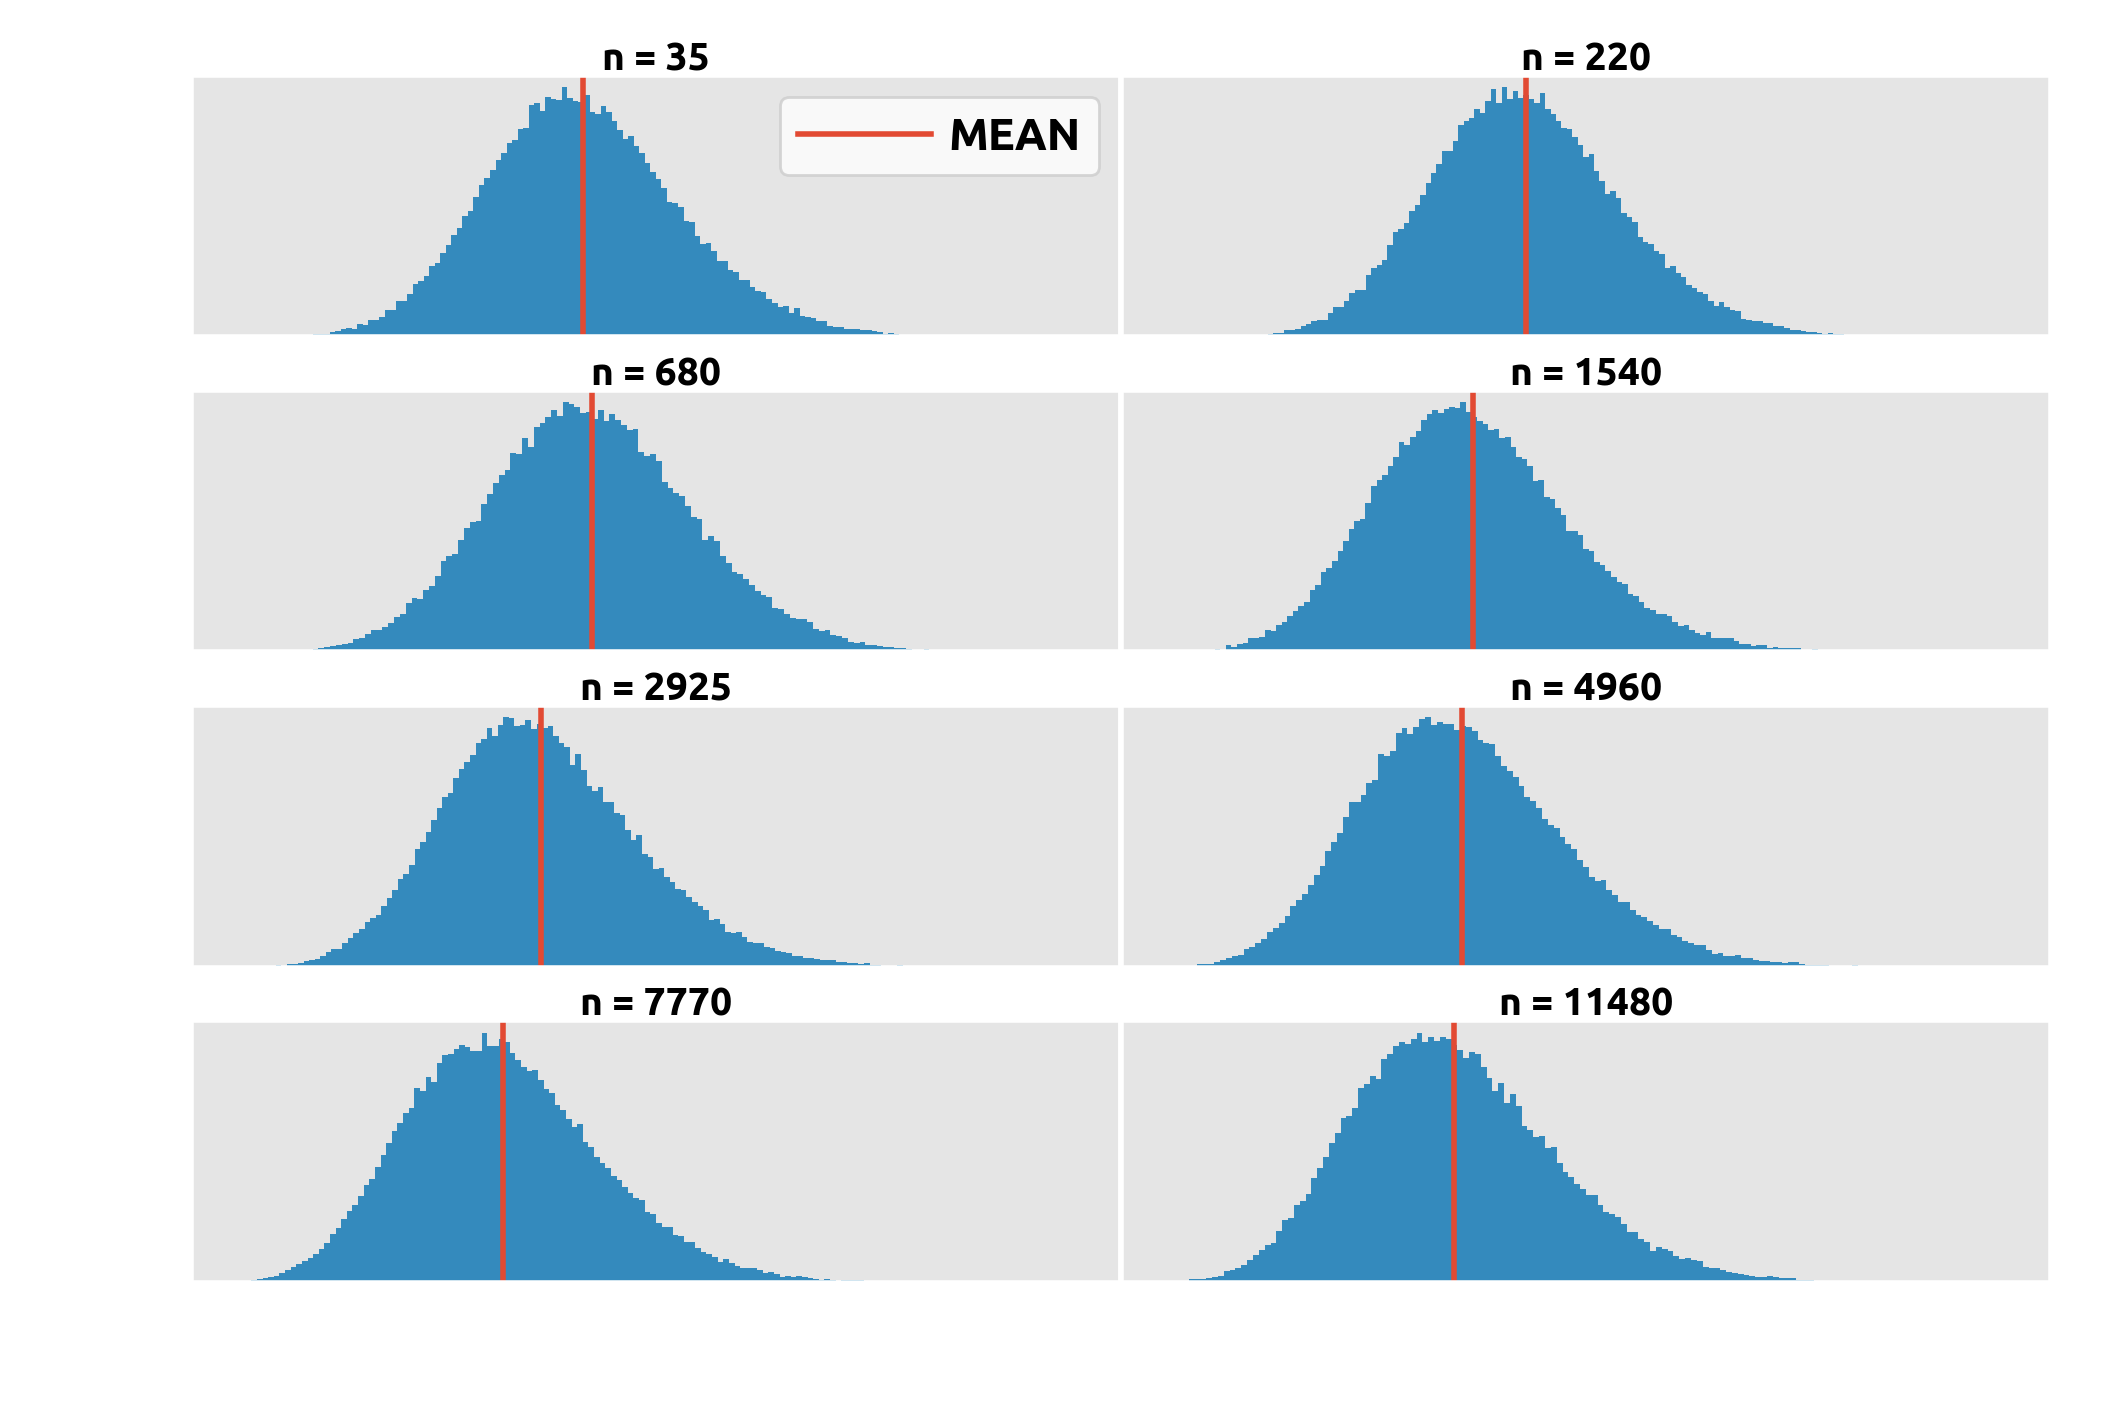
\includegraphics[scale=0.55]{histograms_NORMAL.png}}
	\subfloat[Gamma weights.]{\label{plot.hist_gamma}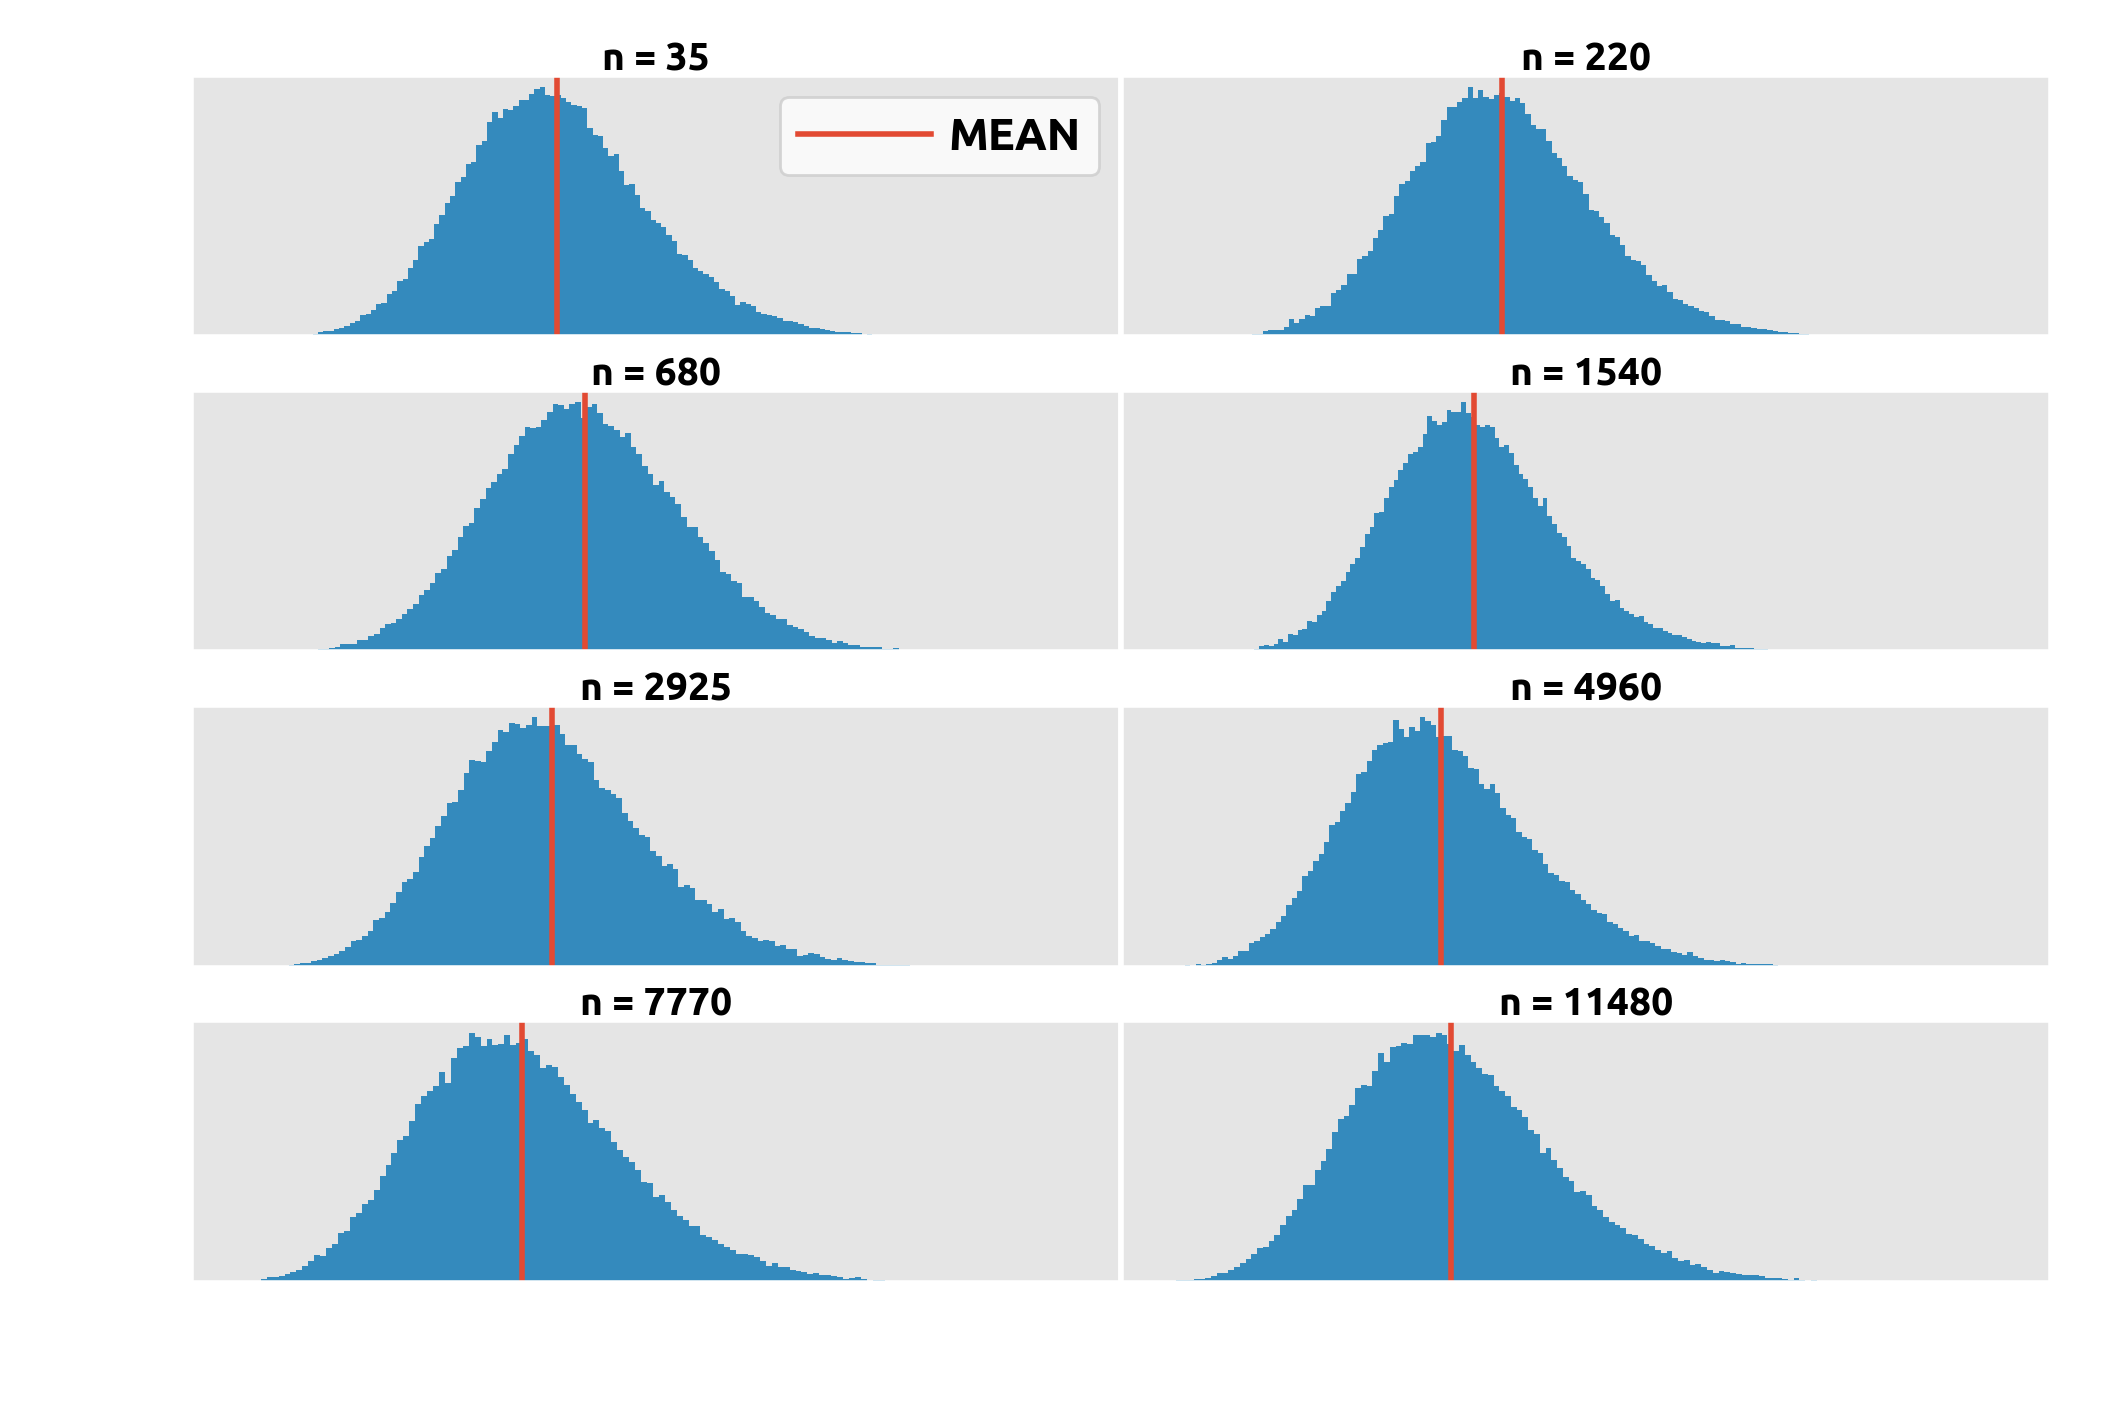
\includegraphics[scale=0.55]{histograms_GAMMA.png}}
	\caption{Visualizations of empirical longest path distributions for Cholesky graphs.}	
	\label{plot.emp_hists} 
      \end{figure}

      \subsubsection{How sensitive is the longest path distribution?}
      \label{subsubsect.sensitive}

      Since the CLT-based heuristics are agnostic of the weight distributions, clearly they will be of little use for a given graph if the longest path distribution can vary widely depending on what distributions the weights follow. Hence it will be helpful going forward to establish how much variation we can expect to see for the graphs in our test sets.

      Figure \ref{plot.emp_hists} shows that the shapes of the Cholesky graphs' empirical longest path distributions are very similar for the two choices of weight distributions considered here. Furthermore, we see from Table \ref{tb.emp_summary} that many summary statistics of the empirical distributions are likewise very close, albeit clearly not identical. For the DAGs in the STG set, we found that the mean and expected value of the empirical distributions were also typically close. Across the entire set of $1620$ graphs, the average difference between mean values for normal and Gamma weights was around $0.5\%$ and never more than $0.7\%$. The average deviation for the variance was more pronounced at about $1.6\%$, with $20$ of the $1620$ graphs recording differences of greater than $5\%$. Of course, this is perhaps to be expected given that these graphs--and therefore the number of summations needed to compute path lengths---are smaller than the majority of those in the Cholesky set.

      To conclude, there will of course always be a range---however narrow---of distributions that the longest path can assume if only the first two moments of the weight distributions are known. However, given the similarities that we have seen for the graphs in our test sets, the weight distribution independence assumption of the CLT approach is fairly reasonable, especially for the Cholesky graphs. Since task timing distributions in our experiments were usually closer to a Gamma distribution than normal, for the remainder of this investigation, when use reference solutions obtained by the MC method, these will have been obtained for Gamma distributed weights. 

\subsubsection{Runtime}
\label{subsubsect.runtime}

Although we have largely avoided discussing runtimes in this thesis so far because our code is not---and is not intended to be---optimal, this is an area in which at least some baseline comparisons are necessary. Table \ref{tb.mc_timings} illustrates how the runtime of our implementation of the MC method increases with the size of the graph and the number of samples for the Cholesky set. The timings presented are for normally distributed weights, as that was always the most efficient of those we considered. Although it is obviously application-specific, one can easily imagine from the data presented in the table how using many samples for the larger graphs may be impractical. 

\begin{table}
	\caption{Time needed for MC implementation for Cholesky graphs.} 
	\begin{center}	
		\begin{tabular}{c c c c c c}
                  \toprule
                  & \multicolumn{5}{c}{\# Samples}     \\
                  \cmidrule{2-6}
                  DAG size & 10 & 100 & 1000 & 10000 & 100000\\
                  \cmidrule{1-6}
                  $35$ & $<0.1$s & $<0.1$s & $0.4$s & $4$s & $41$s\\
                  $220$  & $<0.1$s & $0.5$s & $3$s & $36$s & $5$m $43$s\\
                  $680$ & $0.2$s & $1$s & $12$s & $2$m $9$s & $20$m $44$s\\
                  $1540$ & $0.4$s & $3$s & $32$s & $5$m $22$s & $49$m $56$s\\
                  $2925$ & $0.6$s & $6$s & $1$m $3$s & $10$m $17$s & $1$h $39$m $54$s\\
                  $4960$ & $1$s & $12$s & $1$m $59$s & $17$m $57$s & $2$h $55$m $35$s\\
                  $7770$ & $2$s & $19$s & $3$m $2$s & $29$m $59$s & $4$h $49$m $42$s\\
                  $11480$ & $3$s & $28$s & $4$m $36$s & $46$m $40$s & $7$h $39$m $4$s\\
		\bottomrule
		\end{tabular}
		\label{tb.mc_timings}
	\end{center}	
      \end{table}
      % TODO: Should probably be timings for Gamma weights since that is the reference.

%      Assuming that the longest path distribution is at least roughly normal, it is sufficient to obtain good estimates of its first two moments. This prompts the question: how many samples do we actually need to do this? For the Cholesky DAG set, this was largely a tale of two different moments. Taking the expected values and variances obtained for the full set of $100$,$000$ samples as a reference, we found that, for all of the graphs, the MC method was well within $1\%$ of the expected value after as few as $10$ samples (representing a runtime more than $9000$ times smaller than the full MC method, see Table \ref{tb.mc_timings}). The picture was more complex for the variance, as illustrated in Figure \ref{plot.mc_variance}, but we see that it was usually fairly tight after about 1000 samples as well. Of course, the Cholesky graphs considered here only represent a single family of schedules based on a single application. However, this does serve to demonstrate that it is often possible to converge to the mean and expected value of the longest path distribution after a fairly small number of samples.

      % One speculative approach that might be useful is to consider extreme value theory... The problem is that it isn't clear how to characterize the distribution. Paper by Berman (and other one) seems to suggest that max of dependent normals will also tend to Gumbel but don't know anything about the correlations...
      % More extensive testing with lots of different weight distributions?
      % Comment somewhere about how this is technically a truncated normal but never had to make correction because of the mean and sd values.
      % "There are surely combinations of weight distribution and mean, variance pairs that lead to much more divergent behavior (and DAG topology of course) but for this particular application we're going to take it that they will be extremely similar..."
      % They will however be assumed to be exact in comparisons with other heuristic solutions in later sections.
      % Can probably at least restrict the range of distributions they can follow...

\subsection{Existing bounds and heuristics}
\label{subsect.results_existing}

Several bounds on both the moments and distribution function of the longest path were discussed in Section \ref{sect.bounds}. Given the conclusions of the previous section, from now on we will assume that the longest path distribution is at least roughly normal, so we are most interested in the former. Our experience in the previous chapter with Fulkerson's bound on the expected value suggests that in a scheduling context that approach can be impractically expensive, so we focus here largely on Kamburowski's bounds, since they have also received less attention in the literature. Furthermore, they are the only bounds we are aware of on the variance, which is of clear importance in tandem with the normality assumption. Note that although the bounds technically only hold for normally distributed weights, the CLT suggests that they may still be useful heuristically when that is not the case, since the longest path distribution is likely to be similar in any event, a conclusion largely supported by our results in the previous section. The reference solutions used here assume Gamma weights, so we also evaluate how useful they may be in that case.

Through extensive numerical experiments, Canon and Jeannot showed that the correlation-aware heuristics CorLCA and Cordyn, and the very similar canonical method, all achieved better approximations to the longest path distribution than Sculli's method, on average, for a diverse collection of stochastic graphs. However, they were all more expensive as well. The question is, is the gain in accuracy worth the extra cost in a scheduling context? After all, as we will see in the next chapter, there are examples of stochastic scheduling heuristics that take correlations into account, such as Rob-HEFT \cite{can10}, while there are others that do not, such as {\em stochastic dynamic level scheduling} (SDLS) \cite{li15}. Now, of the three correlation-aware heuristics considered by Canon and Jeannot, CorLCA arguably achieved the best balance of speed and accuracy, so we consider only that as an alternative to Sculli's method here.

Since both heuristics assume that the longest path distribution is normal, in order to evaluate the quality of their solutions we consider the mean and variance estimates separately. This also allows us to compare the quality of the approximations with Kamburowski's bounds. As reference solutions, we use the sample means and variances of the full empirical distributions (with Gamma distributed weights) obtained in Section \ref{subsect.empirical_distribution}; all of the provisos offered there with regards to their quality should therefore always be borne in mind.
% Mention MC30 here and specify it's with normal weights since faster. Assumption is that distribution isn't known so will use the fastest.

\subsubsection{Expected value}
\label{subsubsect.existing_mean}

First, the mean. Table \ref{tb.mean_existing} summarizes the three formal bounds as a percentage of the reference solution for the Cholesky graph set. We see that both lower bounds are very tight. Kamburowski's bound improves on the CPM but the gains are negligible. The upper bound is looser, although even in the worst case it was no more than $19\%$ greater than the true value. Note that despite the fact that the reference solutions do not assume normal weights, both the upper and lower bounds actually hold for all of the graphs.

The heuristic solutions are omitted from the table because they were almost always within $0.1\%$ of the reference mean. Although all three were therefore very good, MC30 was consistently superior to the others; indeed, even the Monte Carlo solution with as few as $10$ samples was more accurate than Sculli's method and CorLCA. It is also interesting to observe that Sculli's method obtained superior estimates than CorLCA for the four largest DAGs. It isn't clear if this is just a fluke because of how close both solutions are to the true mean, or if it suggests that the accumulation of approximation errors can negatively influence CorLCA for larger DAGs.
% Straight to MC30 (which is defined above)?

\begin{table}
	\caption{Bounds on the expected value for Cholesky DAGs, as a percentage of the reference solution.} 
	\begin{center}	
		\begin{tabular}{c c c c c c c c c}
                  \cmidrule{1-9}
                  & \multicolumn{8}{c}{DAG size} \\
                  \cmidrule{2-9}
			& $35$ & $220$ & $680$ & $1540$ & $2925$ & $4960$ & $7770$ & $11480$\\
			\cmidrule{1-9}
			CPM & $99.5$ & $99.1$ & $98.6$ & $98.9$ & $99.2$ & $99.3$ & $99.4$ & $99.5$\\
                  K. lower & $99.9$ & $99.4$ & $98.9$ & $99.2$ & $99.4$ & $99.4$ & $99.5$ & $99.6$\\
                  K. upper & $100.9$ & $104.2$ & $110.3$ & $118.7$ & $116.6$ & $114.1$ & $112.4$ & $111.5$\\
			\bottomrule
		\end{tabular}
		\label{tb.mean_existing}
	\end{center}	
      \end{table}

      Although obviously desirable, the fact that all of the bounds and approximations do so well for the Cholesky set makes evaluating their relative performance difficult. To gauge how they perform in the general case, we repeated the comparison for the STG set. Overall, the comparative performance was somewhat similar, as can be seen from Figure \ref{plot.stg_mean}, which shows the average deviation (in magnitude) from the true mean for the bounds and heuristics across the entire set of $1620$ graphs. However, this time CorLCA is superior on average to Sculli's method and MC30. Furthermore, it obtained better estimates of the mean for $97\%$ and $76\%$ of the graphs, respectively. Note that Kamburowski's upper bound is omitted from the figure as the average deviation was significantly higher than the others at $19\%$. The lower bound however is typically tight, actually providing a better estimate of the mean on average than Sculli's method. As stated above, Kamburowski's bounds do not actually hold here since the reference solution assumes Gamma weights, and they were both occasionally violated: the upper about $0.5\%$ of the time and the lower for just over $7\%$ of DAGs. Violations were also more severe for the lower ``bound'', which in the worst case was actually about $7\%$ greater than the reference solution.     

      \begin{figure}
	\centering	
	\subfloat[Mean.]{\label{plot.stg_mean}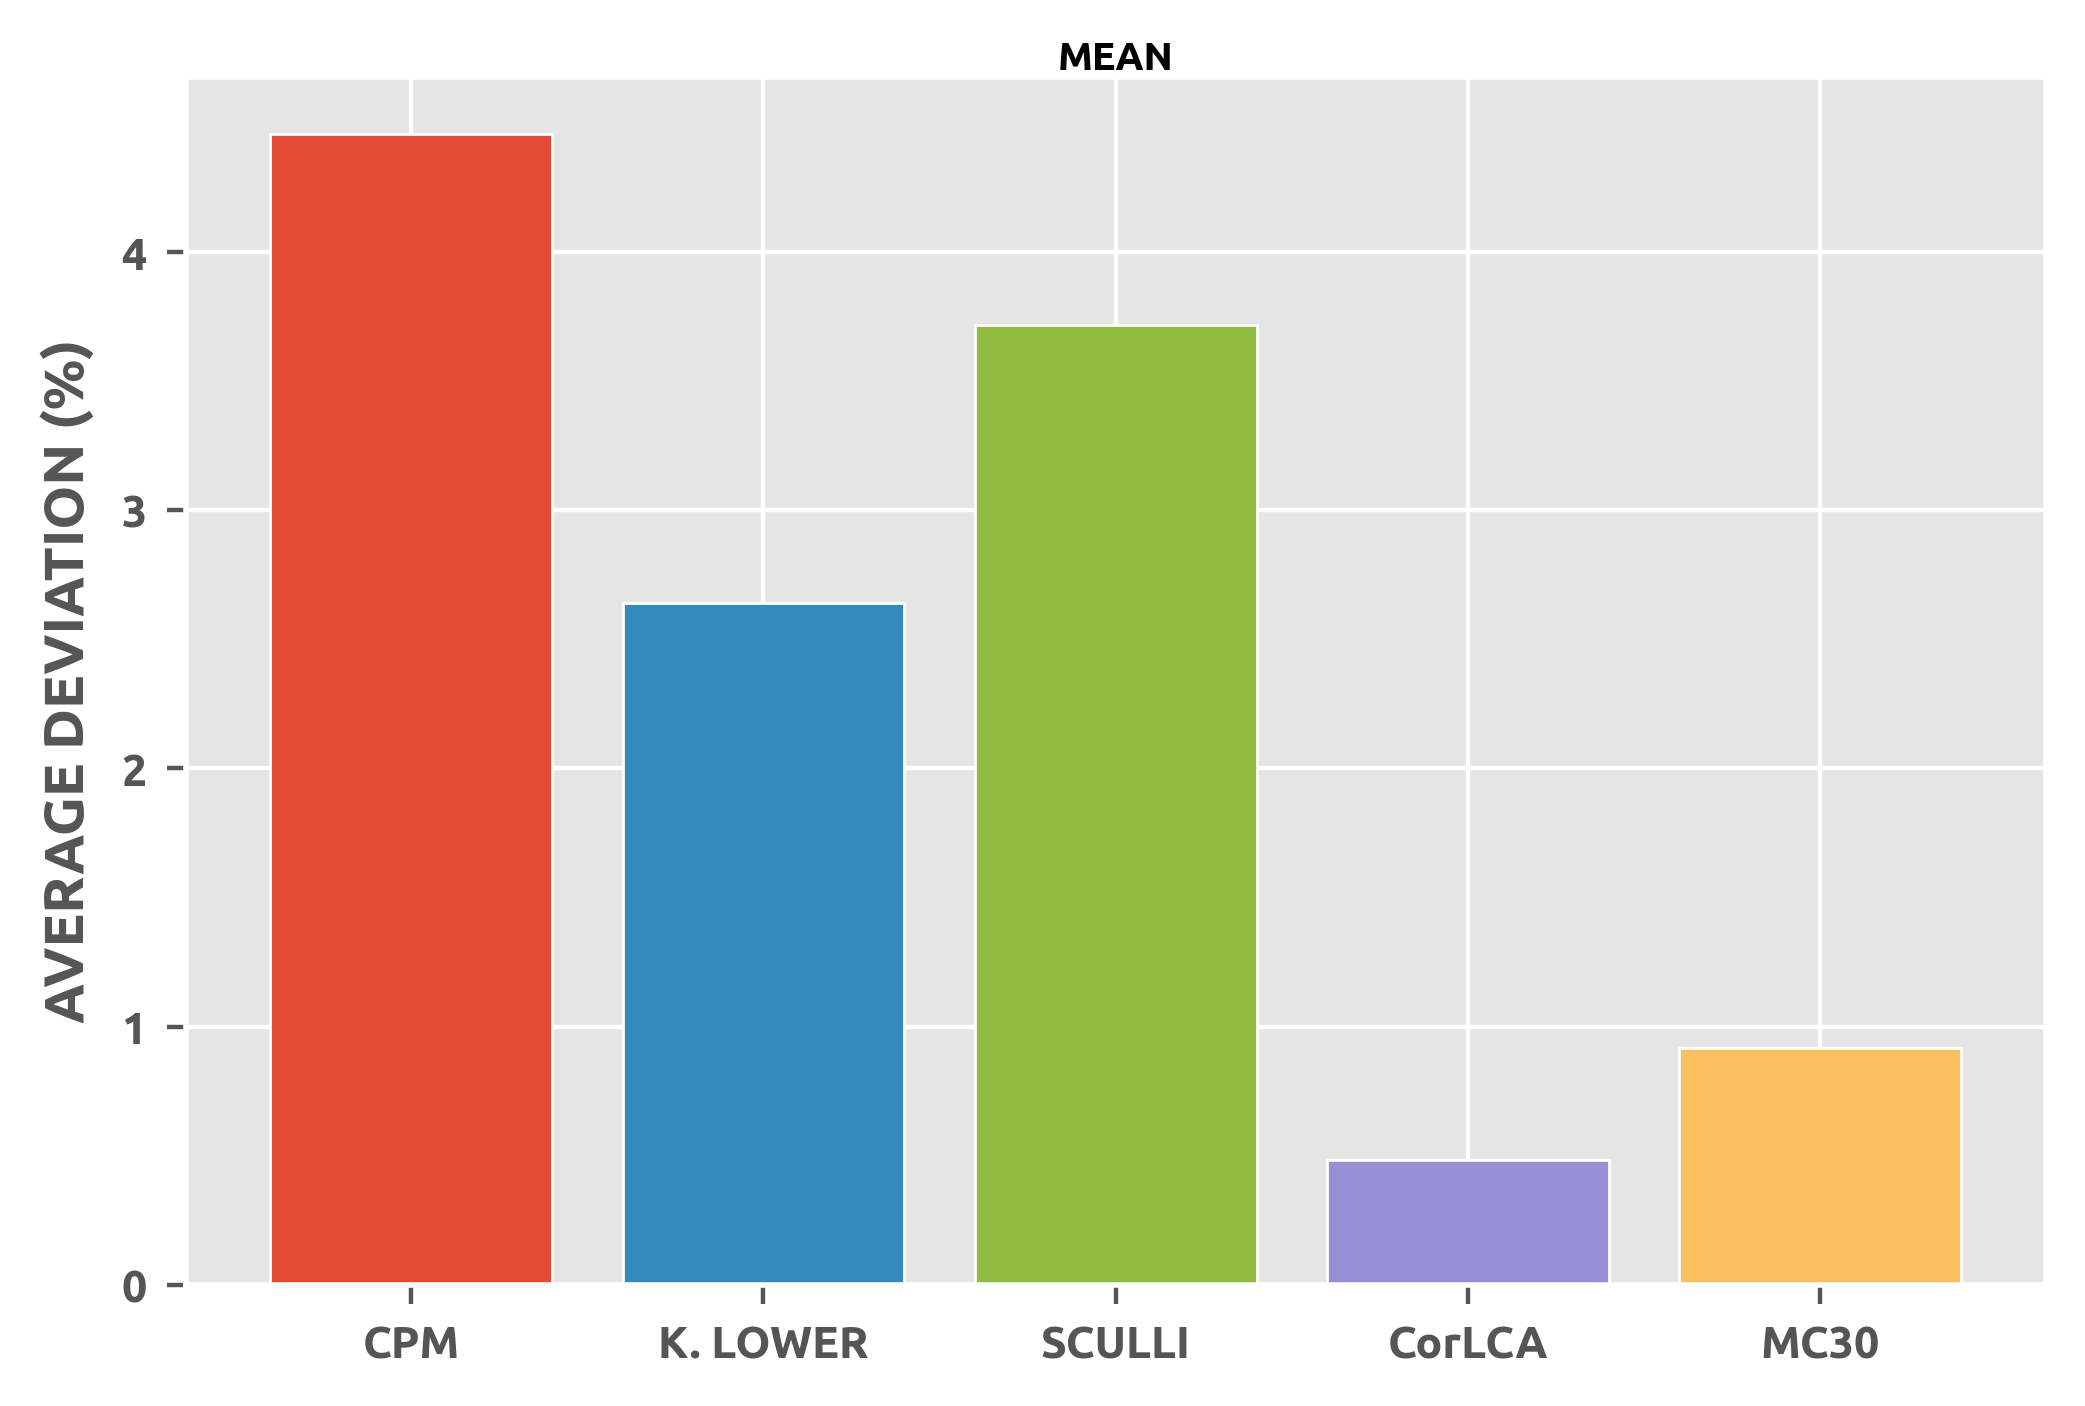
\includegraphics[scale=1.0]{stg_existing_mean.png}}\\
	\subfloat[Variance.]{\label{plot.stg_var}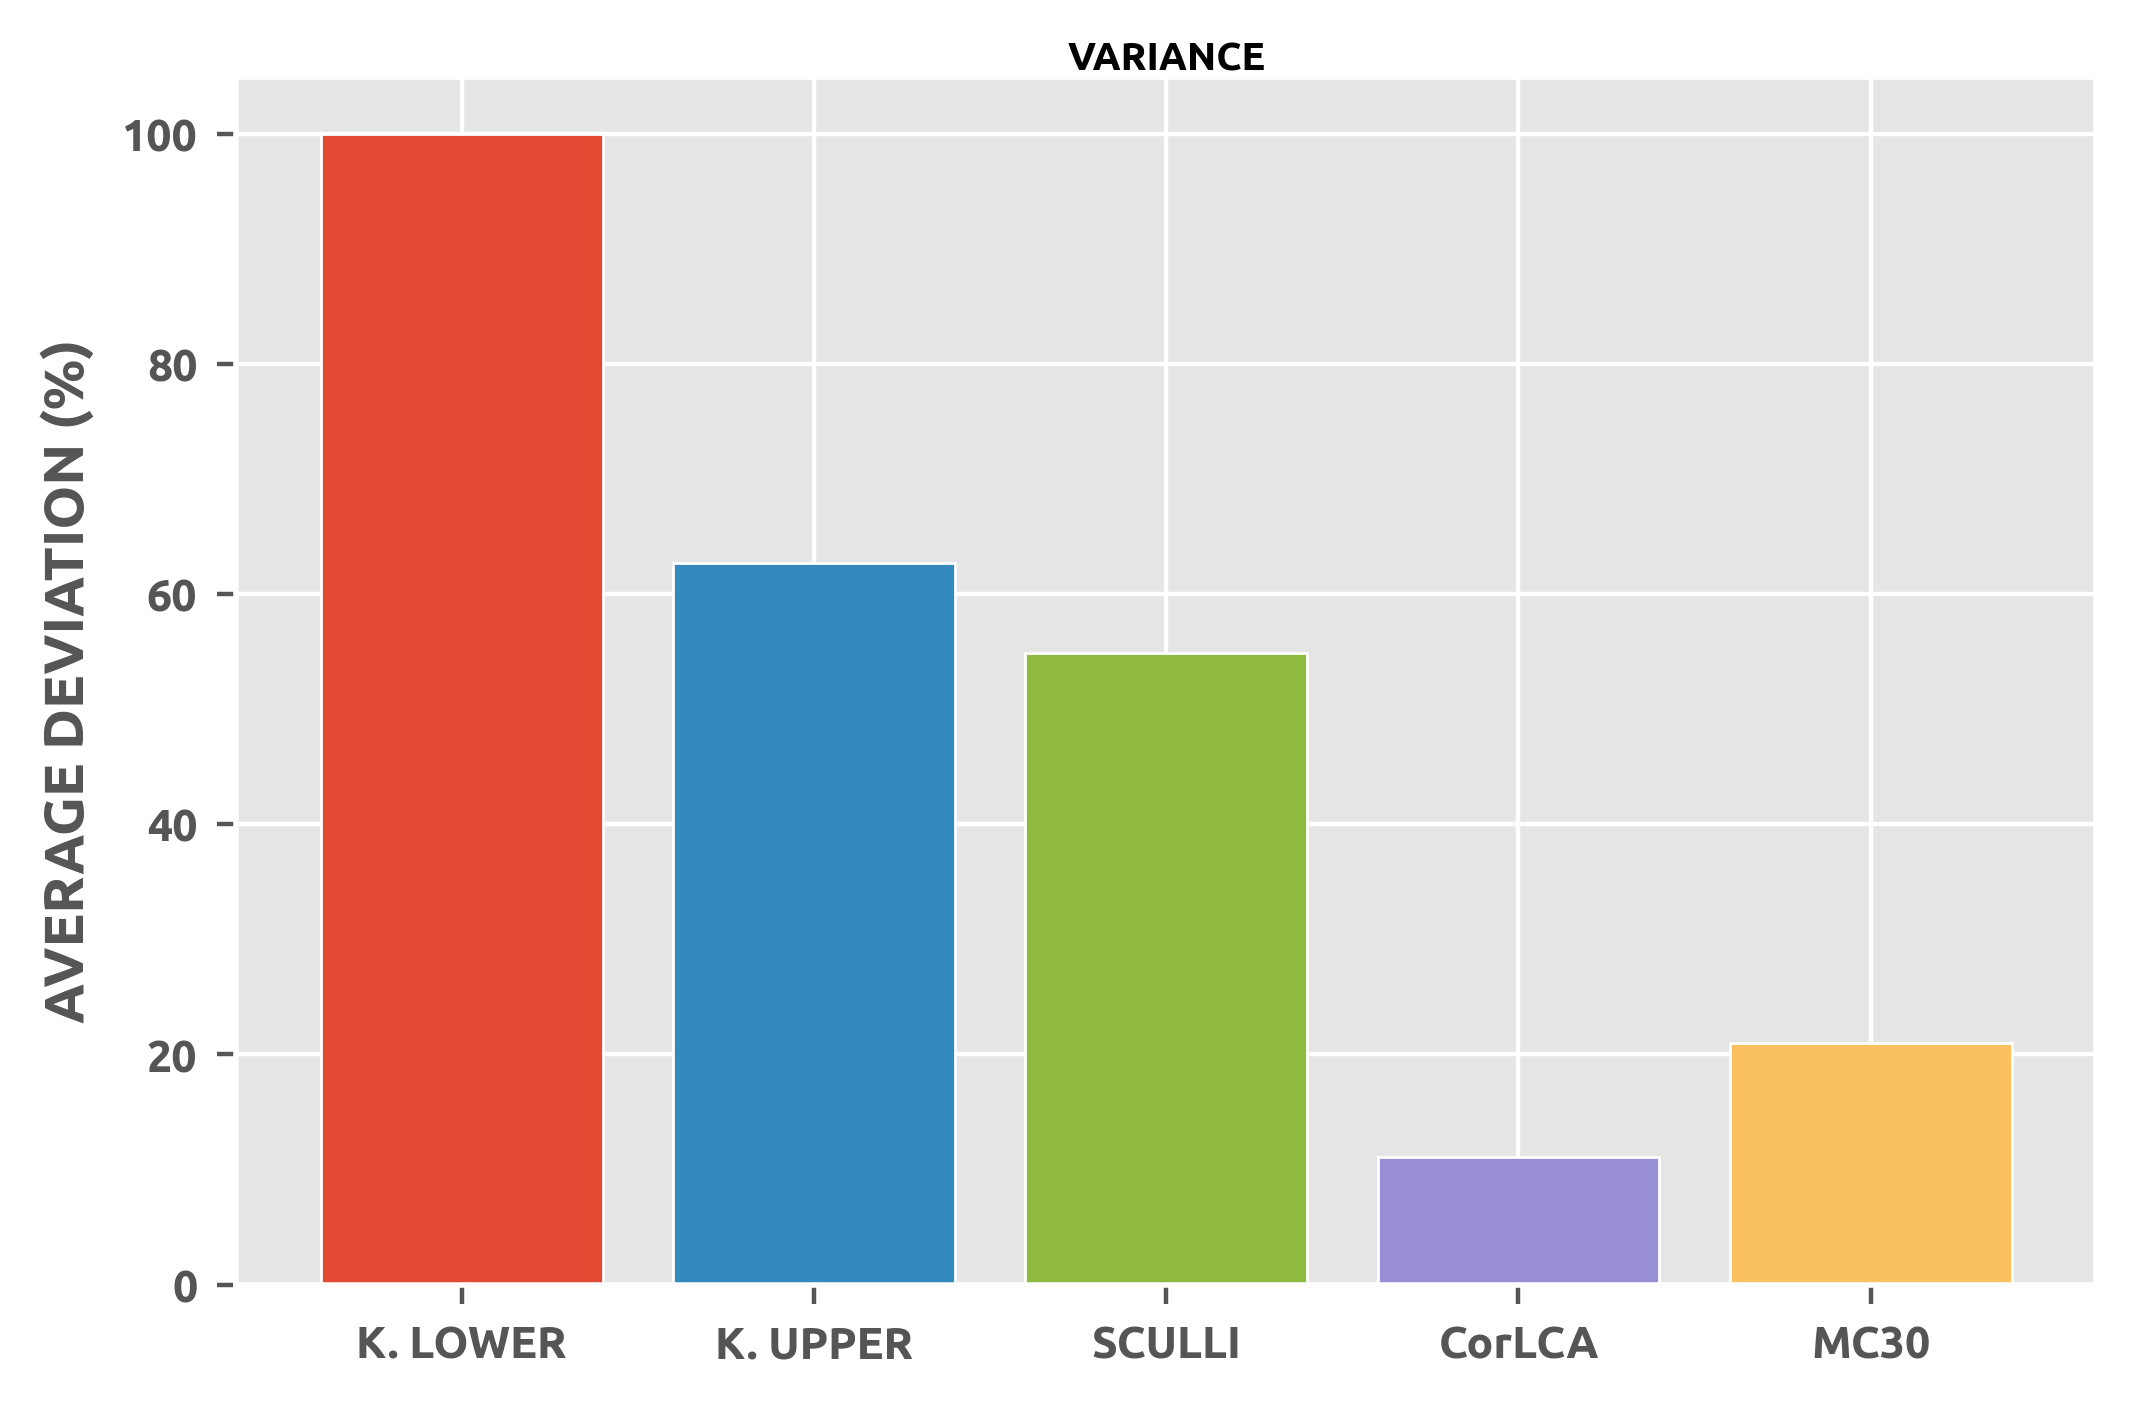
\includegraphics[scale=1.0]{stg_existing_var.png}}
	\caption{Average deviation from reference mean and variance over the STG graph set for bounds and approximations.}	
	\label{plot.stg_mean_var} 
      \end{figure}




      \subsubsection{Variance}
\label{subsubsect.existing_variance}

Unfortunately, the bounds and approximations to the variance were much less accurate than for the mean, as shown for the Cholesky DAGs in Figure \ref{plot.variance_existing} (note the logarithmic scale on the $y$-axis) and the STG graphs in Figure \ref{plot.stg_var}. Kamburowski's lower bound in particular is extremely loose, generally being only about $1\%$ of the true value in all cases. The upper bound is somewhat tighter, although it was still about five times larger than the true value for the Cholesky graphs and on average more than $60\%$ greater for the STG graphs. Depending on the application, these bounds may still be useful but this seems unlikely to be the case when making scheduling decisions. Looking on the bright side, one advantage of their lassitude is that they were almost never violated even though our reference solutions assume Gamma weights: we recorded only seven small violations of the upper bound and none for the lower.
% Violated by how much?

With regard to the heuristics, CorLCA is consistently better than Sculli's method. It also betters MC30 on average for the STG graphs. However, although it does quite well for the smallest three Cholesky DAGs, after this its performance declines, returning variance estimates that are orders of magnitude smaller than the true value for the larger graphs (albeit still better than Sculli's). There are several possible explanations for this apparent poor behavior for large graphs. The simplest is that this is illusory and in fact the problem is that the reference solutions do not represent enough samples to capture the true variance of large graphs. Disregarding this possibility for the moment, the cause could instead be the accumulation of approximation errors when computing maximizations. An observation supporting this is that the variance estimates computed by the forward and backward variants of CorLCA can vary considerably, as shown in Table \ref{tb.corlca_direction}. As noted in Section \ref{sect.path_heuristic}, this effect can perhaps be alleviated by considering paths through the DAG in their entirety, an approach we consider in Section \ref{subsect.results_paths}. 

      \begin{figure}
	\centering	
	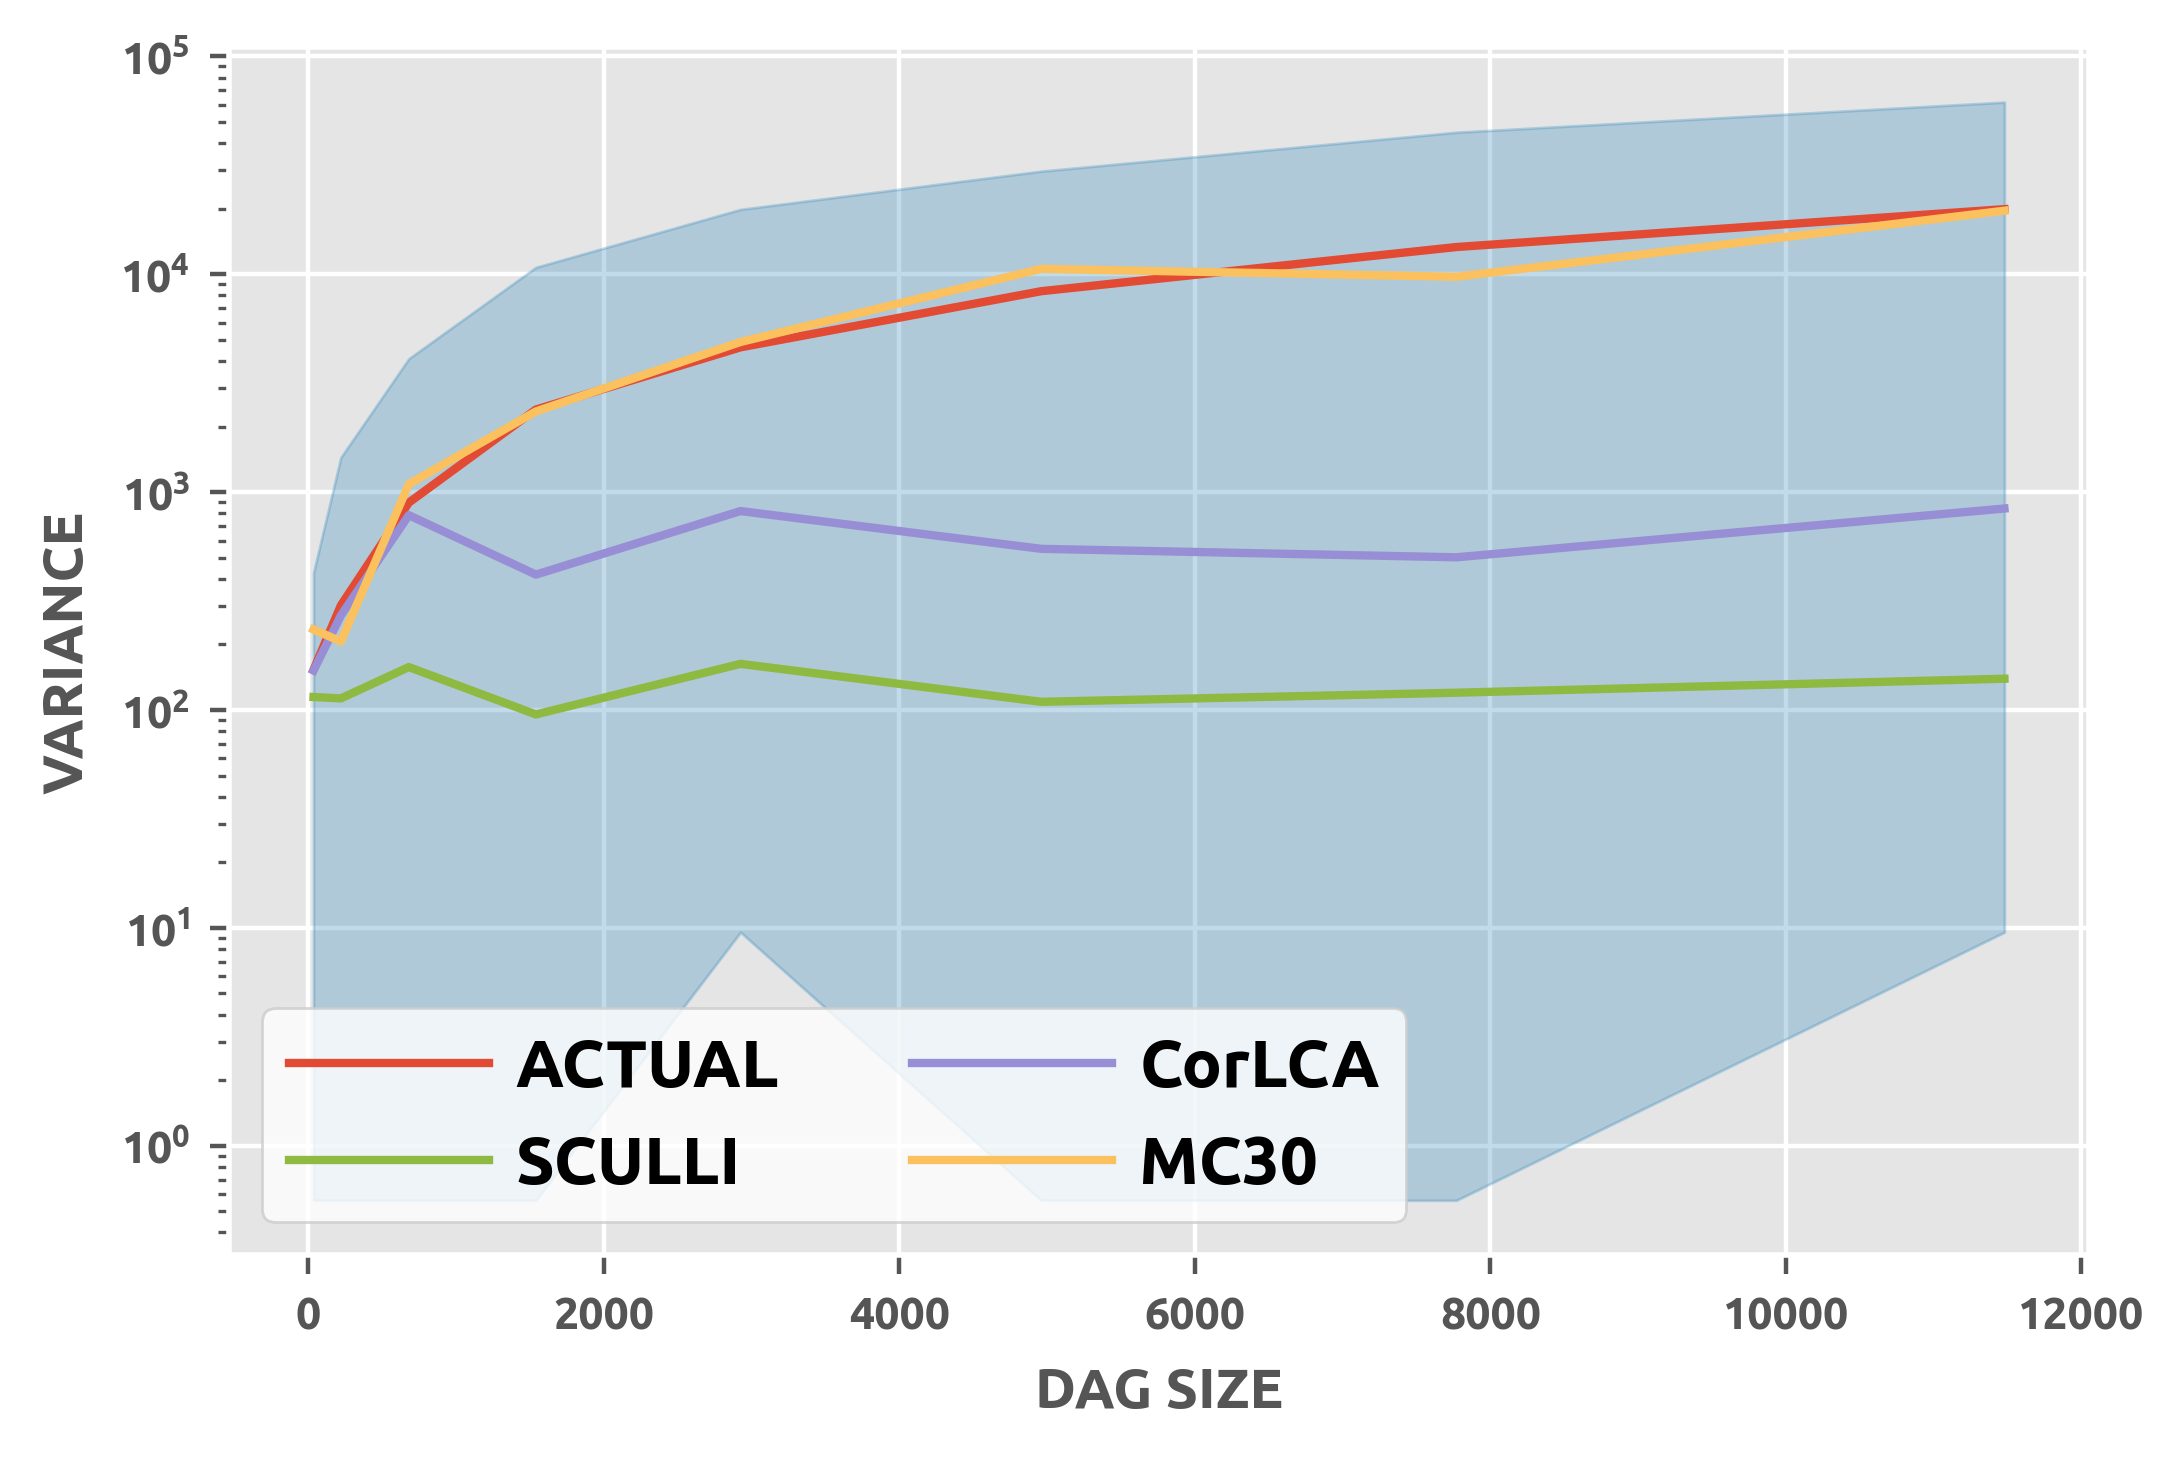
\includegraphics[scale=1.0]{chol_variance.png}
	\caption{Bounds and approximations to the variance for the Cholesky graph set. Blue area defines region within Kamburowski's upper and lower bounds. Solid red line indicates reference solution.}	
	\label{plot.variance_existing}
      \end{figure}
      %MC30 denotes the Monte Carlo solution with 30 realizations.

      \begin{table}
	\caption{Variance estimates for Cholesky DAGs computed by forward and backward variants of CorLCA.} 
        \begin{center}	
        	\begin{tabular}{c c c c}
                  \toprule
                  DAG size & Reference & Forward & Backward \\
                  \cmidrule{1-4}
                  $35$ & $153.0$ & $151.8$ & $152.8$\\
                  $220$ & $302.0$ & $271.5$ & $219.2$ \\
                  $680$ & $895.3$ & $784.2$ & $482.0$\\
                  $1540$ & $2393.9$ & $418.4$ & $704.7$ \\
                  $2925$ & $4621.6$ & $819.1$ & $878.5$ \\
                  $4960$ & $8363.6$ & $549.5$ & $1137.9$ \\
                  $7770$ & $13342.4$ & $502.4$ & $1243.6$ \\
                  $11480$ & $19913.2$ & $841.3$ & $1419.2$ \\
        	\bottomrule
        	\end{tabular}
        	\label{tb.corlca_direction}
        \end{center}	
      \end{table}

      \subsubsection{Practical considerations}
\label{subsubsect.existing_practical}

      Of course, as well as accuracy, the other key consideration when evaluating bounds and approximations is how long they take to compute. As always, this depends to an extent on the details of the implementation but for what it's worth, in Figure \ref{plot.chol_existing_timings} we illustrate the runtimes of our own. We see that computing the bounds is consistently more expensive than either of the heuristics, typically taking about twice as long as Sculli's method in particular. It should however be noted that the mean bounds depend on the variance bounds but not vice versa; the former are much more expensive since they require repeated evaluation of the unit normal cdf, so if only the variance is required then the runtime would be considerably reduced. Given that the mean estimates achieved by the heuristics are typically very good but the variances less so, this might be a practical option. With regard to the two heuristics, CorLCA was on average about $15\%$ more expensive than Sculli's method. Given the relatively small benefits observed for the Cholesky DAG set as a whole, overall we must conclude that the additional cost does not appear to be worthwhile. However, for the three smallest DAGs significant gains were apparent with regards to the variance, so again a more thorough experimental investigation may be warranted.  

      \begin{figure}
	\centering	
	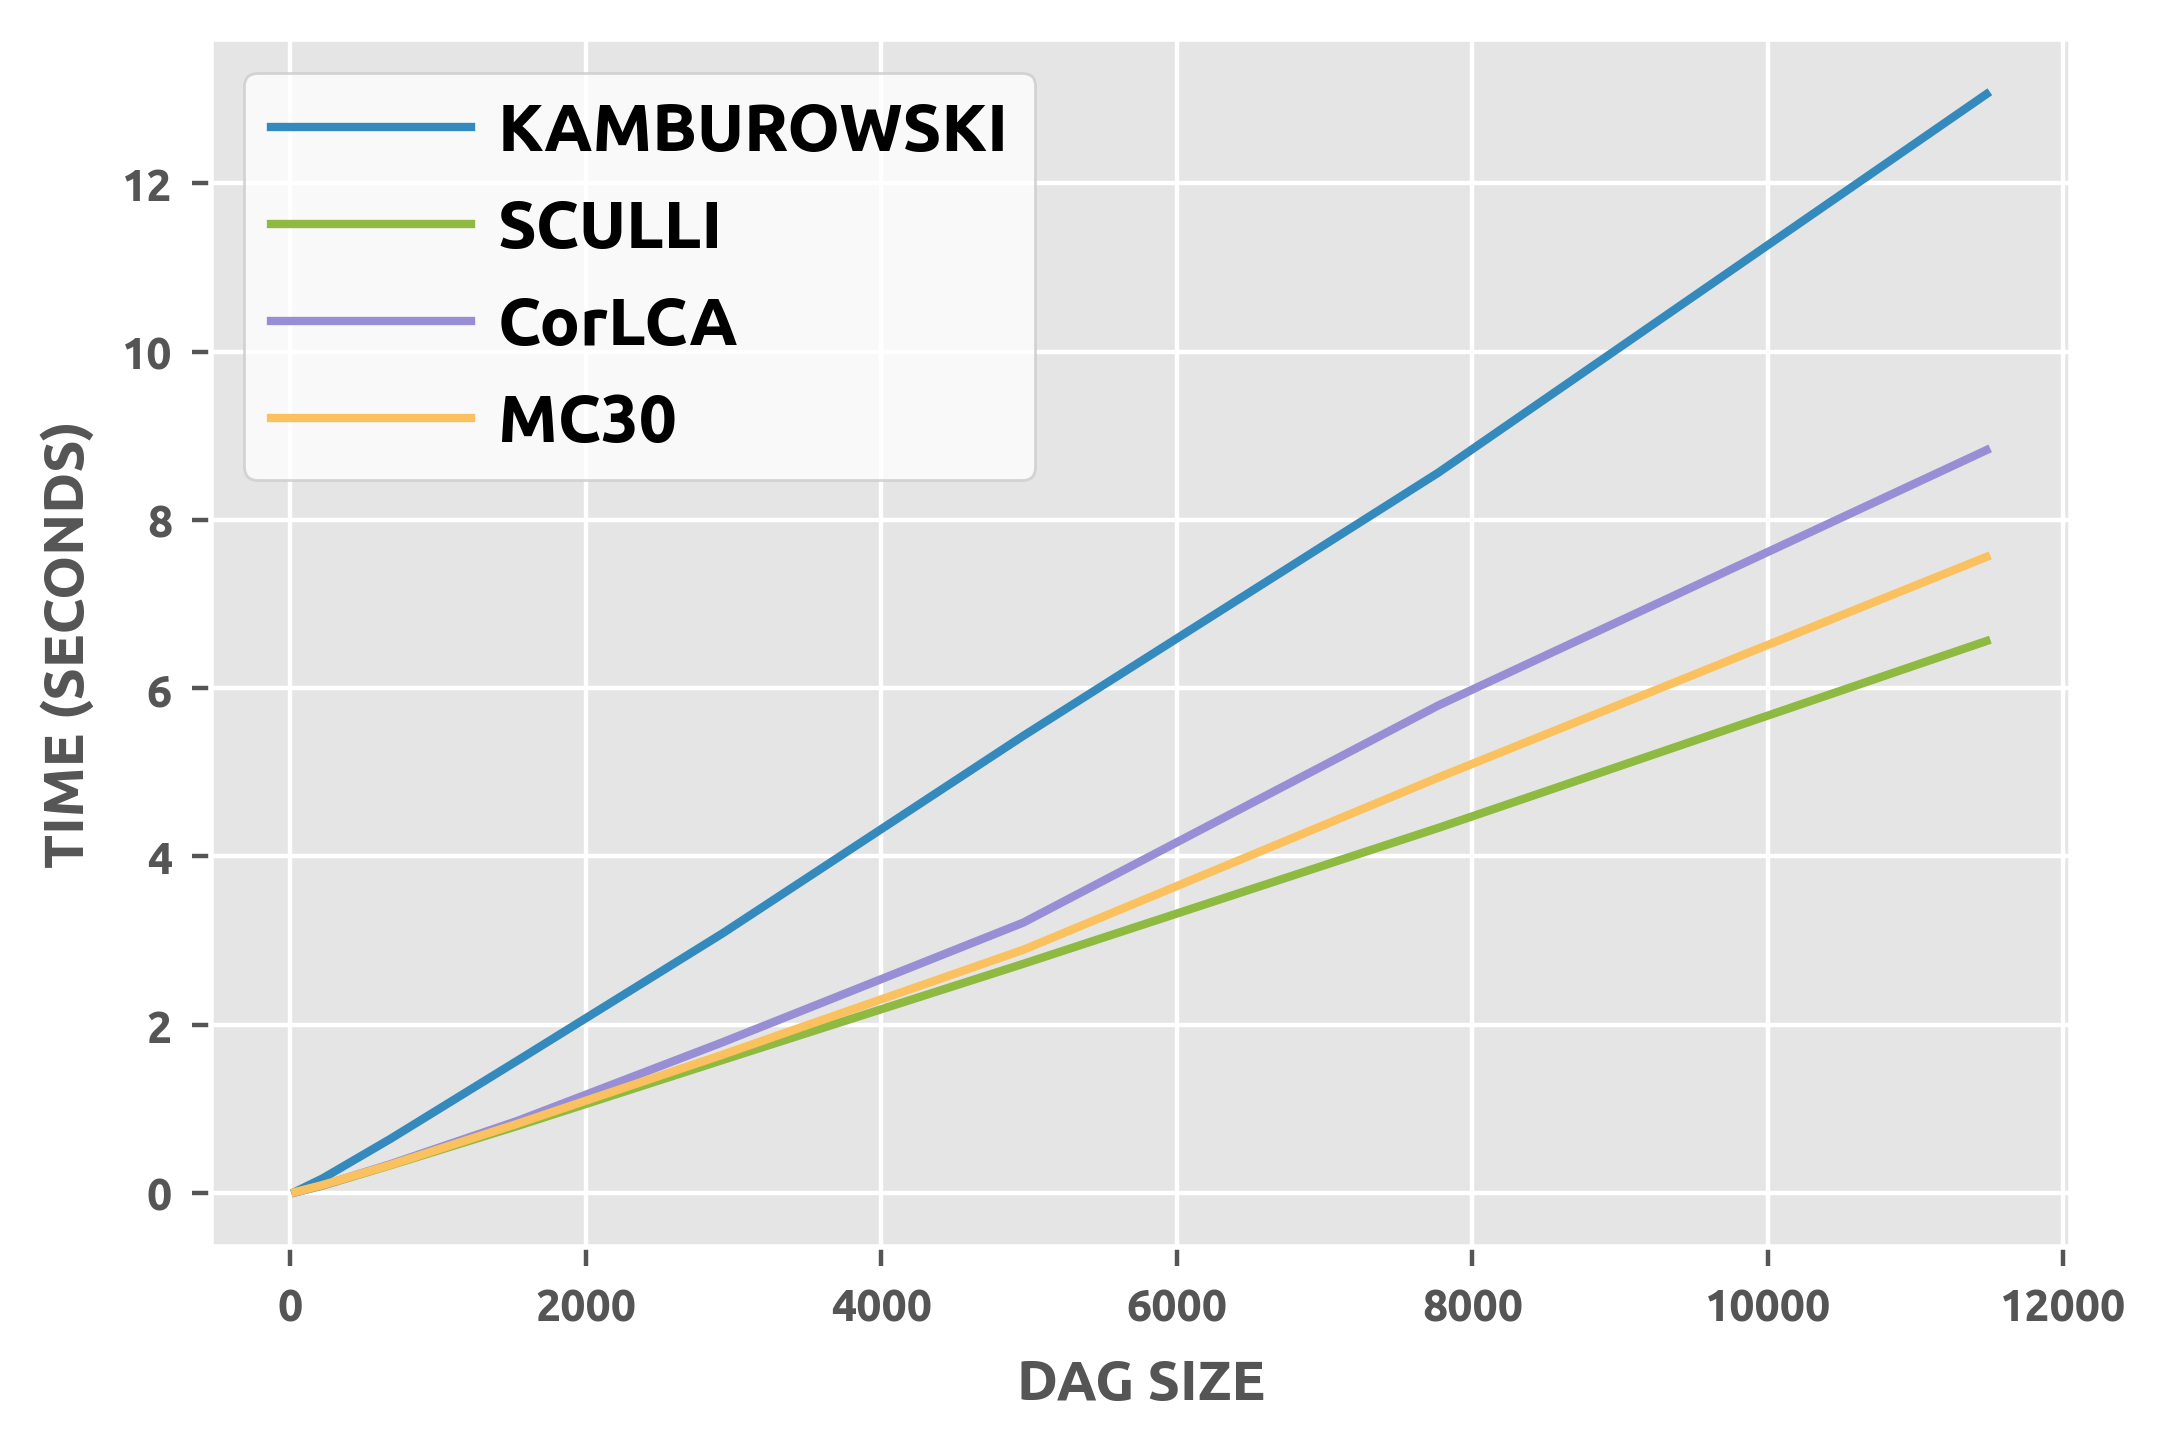
\includegraphics[scale=1.0]{chol_existing_timings.png}
	\caption{Runtimes for Kamburowski's bounds, Sculli's method and CorLCA.}	
	\label{plot.chol_existing_timings}
      \end{figure} 

% One of the advantages is supposed to be if we don't know the distribution, but note that the CLT also says it doesn't matter so we can just take them to be normal. 
% (note the logarithmic scale on the $y$-axis)

\subsection{Path reduction}
\label{subsect.results_paths}

Compare path based alternatives...

\subsection{Updating the finish time}
\label{subsect.results_updating}

Consider different permutations (fraction of tasks initially realized, distributions of the costs, etc) in a systematic manner and compare with MC estimates... 

\section{Conclusions}
\label{sect.conclusions}

Conclusions go here. 

%%%%%%%%%%%%%%%%%%%%%%%%%%%%%%%%%%%%%%%%%%%%%%%%%%%%%%%%%%%%%%%%%%%%%%%%%%%%%%%%%%%%%%%%%%%%
% Bibliography.
%%%%%%%%%%%%%%%%%%%%%%%%%%%%%%%%%%%%%%%%%%%%%%%%%%%%%%%%%%%%%%%%%%%%%%%%%%%%%%%%%%%%%%%%%%%%
\bibliographystyle{myplain2-doi}
\bibliography{references,strings}

\end{document}

%%% Local Variables:
%%% mode: latex
%%% TeX-master: t
%%% End:
